\section{Differentiation} 

  In general, there are two ways that we define a derivative: as a limit and with infinitesimals. In a standard analysis course, we introduce the derivative as the limit of the difference quotient $\Diff_h f(x) = \frac{f(x + h) - f(x)}{h}$. However, there is a second definition that emphasizes the existence of a best linear approximation. This is an equivalent definition and has two advantages. First, a lot of physicists tend to use this formulation, and second, it frames the derivative of one-variable functions well so that it is easy to generalize into Frechet derivatives for multivariate functions. Therefore, I think it is best to introduce them concurrently. Furthermore, these two formulations each naturally lead to the Taylor's theorems with Lagrange and Peano forms of the remainder. Later in measure theory, we will see another type of derivative called the \hyperref[mt-def:dini-der]{Dini derivative}, which is yet generalization designed to be as ``bullet-proof'' as possible. 

  These two are equivalent definitions since the following two different quotients $\phi(y) = \frac{f(x) - f(y)}{x - y}$ and $\gamma(h) = \frac{f(x + h) - f(x)}{h}$ are related in the sense that $\phi(y) = \gamma(y - x)$. So the following two limits exist or fail to exist simultaneously. If they do both exist, then $\lim_{y \to x} \phi(y) = \lim_{y \to x} \gamma(y - x) = \lim_{y \to 0} \gamma(y) = \lim_{h \to 0} \gamma(h)$ where the only nontrivial equality is the second equality, which is true (should be shown). 

  \begin{definition}[Derivative]
    Let $f: E \subset \mathbb{R} \to \mathbb{R}$ and $x \in \mathbb{R}$ be a limit point of $E$. $f$ is said to be \textbf{differentiable at $x$} if it satisfies either of the equivalent definitions. 
    \begin{enumerate}
      \item \textit{Limit Definition}. If the following limit exists in $\mathbb{R}$.
        \begin{equation}
          f^\prime (x) \coloneqq \lim_{h \to 0} \frac{f(x + h) - f(x)}{h} = \lim_{y \to x} \frac{f(y) - f(x)}{y - x} \label{lim_def}
        \end{equation}

      \item \textit{Fundamental Increment Lemma}. If there exists a number $f^\prime (x) \in \mathbb{R}$ s.t. 
        \begin{equation}
          f(x + h) - f(x) = f^\prime (x) h + o(h)
        \end{equation}
        We call the mapping $df(x) : h \to f^\prime (x) h$ the \textbf{differential} of $f$ at $x$. 
    \end{enumerate}
    If $f$ is differentiable at $x$, then we call $f^\prime(x) \in \mathbb{R}$ the \textbf{derivative of $f$ at $x$}. If $f$ is differentiable for all $x \in [a, b]$, we say $f$ is \textbf{differentiable on $[a, b]$}. 

    \begin{figure}[H]
      \centering 
      \begin{tikzpicture}[>=Stealth, scale=0.7, thick, font=\small]
        % --- Define parameters and functions ---
        % These control the shape of the curve and the positions of the points.
        \def\xval{2.5}    % The x-coordinate
        \def\hval{3.0}    % The step size h
        \def\xhval{\xval + \hval} % x + h

        % Define the function f(x). A quadratic gives a good convex shape.
        % f(x) = 0.15 * x^2 + 1
        \def\f(#1){0.15*(#1)^2 + 1}
        % Define the derivative f'(x).
        % f'(x) = 2 * 0.15 * x = 0.3 * x
        \def\fp(#1){0.3*(#1)}

        % --- Calculate key coordinates ---
        \pgfmathsetmacro{\yval}{\f(\xval)}           % f(x)
        \pgfmathsetmacro{\yhval}{\f(\xhval)}         % f(x+h)
        \pgfmathsetmacro{\slope}{\fp(\xval)}         % f'(x)
        \pgfmathsetmacro{\ytanval}{\yval + \slope*\hval} % f(x) + f'(x)h

        % Define coordinate points
        \coordinate (O) at (0,0);
        \coordinate (X) at (\xval, 0);
        \coordinate (XH) at (\xhval, 0);
        \coordinate (P) at (\xval, \yval);          % Point on curve at x
        \coordinate (Q) at (\xhval, \yhval);        % Point on curve at x+h
        \coordinate (PTan) at (\xhval, \ytanval);   % Point on tangent at x+h
        \coordinate (Corner) at (\xhval, \yval);    % Corner of the dy/dx triangle

        % --- Draw Axes ---
        \draw[->, line width=1pt] (-1,0) -- (7.5,0);
        \draw[->, line width=1pt] (0,-1) -- (0,6.3);

        % --- Draw Ticks and Labels on Axes ---
        % X-axis
        \draw (\xval, 3pt) -- (\xval, -3pt) node[below, yshift=-2pt] {$x$};
        \draw (\xhval, 3pt) -- (\xhval, -3pt) node[below, yshift=-2pt] {$x+h$};

        % Y-axis
        \draw (3pt, \yval) -- (-3pt, \yval) node[left, xshift=-2pt] {$f(x)$};
        \draw (3pt, \yhval) -- (-3pt, \yhval) node[left, xshift=-2pt] {$f(x+h)$};
        \draw[blue] (3pt, \ytanval) -- (-3pt, \ytanval) node[left, xshift=-2pt] {$f(x) + f^\prime(x) \, h$};

        % --- Draw the Function and Tangent Line ---
        % Function f
        \draw[line width=1.2pt] plot[domain=-0.5:6.0, smooth] (\x, {\f(\x)}) node[above left, xshift=-5pt] {\Large $f$};

        % Tangent line df(x)
        % Calculate start and end points for the tangent line segment
        \coordinate (TanStart) at ($(P) - (1.5, {1.5*\slope})$);
        \coordinate (TanEnd) at ($(PTan) + (1.0, {1.0*\slope})$);
        \draw[blue, line width=1.2pt, <->] (TanEnd) -- (TanStart) node[below, yshift=2pt] {$df(x)$};

        % --- Draw Projection Lines ---
        \draw[gray!50, thin] (X) -- (P);
        \draw[gray!50, thin] (XH) -- (Q);
        \draw[gray!50, thin] (0, \yval) -- (P);
        \draw[gray!50, thin] (0, \yhval) -- (Q);
        \draw[blue!30, thin] (0, \ytanval) -- (PTan); % Blueish horizontal line
        \draw[gray!50, thin] (P) -- (Corner);         % Horizontal part of the triangle

        % --- Draw Points ---
        \fill (P) circle (2pt);
        \fill (Q) circle (2pt);
        \fill (Corner) circle (2pt);
        \fill (PTan) circle (2pt);

        % df(x)(h) (Blue vertical segment and label)
        \draw[blue, line width=1.5pt] (Corner) -- (PTan);
        \node[blue, right] (dflabel) at ($(Corner)!0.5!(PTan) + (1.5,0)$) {$f^\prime (x)\,h$};
        \draw[blue, ->, thick] (dflabel.west) -- ($(Corner)!0.5!(PTan)$);

        % d(x;h) (Red vertical segment and label)
        \draw[red, line width=1.5pt] (PTan) -- (Q);
        \node[red, right] (dlabel) at ($(PTan)!0.5!(Q) + (1.5,0)$) {$o(h)$};
        \draw[red, ->, thick] (dlabel.west) -- ($(PTan)!0.5!(Q)$);
      \end{tikzpicture}
      \caption{The graph of the differential $df(x): h \mapsto f^\prime (x) h$ is the best linear approximation of $f$ around $x$, i.e. the tangent line. Note that the difference (in red) is the function $\varphi(h) = f(x + h) - f(x) - f^\prime(x) h \in o(h)$. } 
      \label{fig:differential_diagram}
    \end{figure}
  \end{definition} 
  \begin{proof}
    We prove bidirectionally. 
    \begin{enumerate}
      \item $(\rightarrow)$. Let us define $\varphi(h) = f(x + h) - f(x) - f^\prime (x) h$. We claim that this is $o(h)$, since 
        \begin{align}
          \lim_{h \to 0} \frac{\varphi(h)}{h} & = \lim_{h \to 0} \bigg( \frac{f(x + h) - f(x) - f^\prime (x) h }{h}\bigg) \\  
                                              & = \lim_{h \to 0} \bigg( \frac{f(x + h) - f(x)}{h} - f^\prime (x) \bigg) \\  
                                              & = \lim_{h \to 0} \bigg( \frac{f(x + h) - f(x)}{h} \bigg) - f^\prime (x)  \\  
                                              & = f^\prime(x) - f^\prime(x) = 0 
        \end{align}
        Therefore, we can verify that 
        \begin{equation}
          f^\prime (x) h + \varphi(h) = f^\prime (x) h + f(x + h) - f(x) - f^\prime (x) h = f(x + h) - f(x)
        \end{equation}

      \item $(\leftarrow)$. Assume such a $f^\prime (x)$ and $\varphi(h)$ exist. Then, we can see that by dividing both sides by $h$. 
        \begin{equation}
          \frac{f(x + h) - f(x)}{h} = f^\prime(x) + \frac{\varphi(h)}{h} 
        \end{equation}
        We must throw away the case where $h = 0$ since we divided by $h$, but it doesn't matter since we are taking the limit as $h \to 0$. 
        \begin{align}
          \lim_{h \to 0} \frac{f(x + h) - f(x)}{h} & = \lim_{h \to 0} \bigg( f^\prime (x) + \frac{\varphi(h)}{h} \bigg) \\ 
                                                   & = f^\prime (x) + \lim_{h \to 0} \frac{\varphi(h)}{h} \\ 
                                                   & = f^\prime(x) + 0 = f^\prime(x)
        \end{align}
    \end{enumerate}
  \end{proof} 

  Therefore, we call the derivative also the \textit{best linear approximation} of the function $f$. With this, we can establish the fun fact of the origins of \textit{Leibniz's notation} of the derivative. Consider the identity function $\iota: x \mapsto x$, and denote its differential $dx (h) = d\iota (h) = h$. Then, for any differentiable function, we can do 
  \begin{equation}
    df(x)(h) = f^\prime (x) \, h = f^\prime (x) \, dx(h)
  \end{equation}
  where the first equality follows from the definition and the second equality comes from substituting $dx(h) = h$ in it. Now removing the input parameter $h$, we have 
  \begin{equation}
    df(x) = f^\prime (x) dx \implies \frac{df(x)}{dx} = f^\prime (x)
  \end{equation}
  Therefore, the ``fraction'' on the left hand side is really just a fraction of two functions of $h$! It turns out that since $df(x)$ is linear, the $h$'s in the numerator and denominator cancels out, and the fraction reduces to a constant. 

  Note that I've been very careful with this definition. A lot of authors use the fact that $f$ must be defined on an open set $U$ and choose $x \in U$. However, this might be restrictive in cases where we want to look at ``derivatives'' on boundaries. Our definition is a generalization of that since if $x$ is indeed in the interior of $E$, then Equation \ref{lim_def} by \hyperref[def:lim-func]{definition of the limit of a function} becomes a two-sided limit. If $x$ is on the boundary of $E$, then this is still well-defined as a one-sided derivative. We also adopt the convention from limits that a function may be right or left differentiable, which is useful as I've seen it pop up a few times here and there. 

  \begin{definition}[One-Sided Derivative]
    Let $f: E \subset \mathbb{R} \to \mathbb{R}$. 
    \begin{enumerate}
      \item If $x$ is a limit point of $E \cap [x, +\infty)$, then the following limit---if it exists---is called the \textbf{right derivative of $f$ at $x$}. 
        \begin{equation}
          f^\prime_+ (x) = \lim_{y \to x^+} \frac{f(y) - f(x)}{y - x}
        \end{equation}

      \item If $x$ is a limit point of $E \cap (-\infty, x]$, then the following limit---if it exists---is called the \textbf{left derivative of $f$ at $x$}. 
        \begin{equation}
          f^\prime_- (x) = \lim_{y \to x^-} \frac{f(y) - f(x)}{y - x}
        \end{equation}
    \end{enumerate}
  \end{definition}

  \begin{lemma}[Differentiability Implies Continuity]
    If $f$ is differentiable at $x$, it is continuous at $x$. 
  \end{lemma}
  \begin{proof} 
    If $f$ is differentiable at $x$, then the derivative 
    \begin{equation}
      f^\prime (x) = \lim_{y \to x} \frac{f(x) - f(y)}{x - y} 
    \end{equation}
    exists. Therefore, 
    \begin{align}
      0 = f^\prime (x) \cdot 0 & = f^\prime (x) \big( \lim_{y \to x} x - y \big) \\
                               & = \lim_{y \to x} \frac{f(x) - f(y)}{x - y} \cdot \lim_{y \to x} x - y \\
                               & = \lim_{y \to x} \frac{f(x) - f(y)}{x - y} (x - y) \\
                               & = \lim_{y \to x} f(x) - f(y)
    \end{align}
    which implies that $f(x) = \lim_{y \to x} f(y)$, and hence $f$ is continuous at $x$. 
  \end{proof} 

  Therefore, we can see that the set of differentiable functions is a subset of the set of continuous functions.  

\subsection{Rules of Differentiation}

  \begin{lemma}[Arithmetic]
    If $f$ and $g$ are differentiable at $x$, then 
    \begin{enumerate}
      \item \textit{Linearity}. $f + g$ is differentiable at $x$ with 
        \begin{equation}
          (f + g)^\prime (x) = f^\prime (x) + g^\prime (x)
        \end{equation}
      \item \textit{Product Rule}. $fg$ is differentiable at $x$ with 
        \begin{equation}
          (fg)^\prime (x) = f^\prime (x) g(x) + f(x) g^\prime (x)
        \end{equation}
      \item \textit{Quotient Rule}. $f/g$ is differentiable at $x$ with 
        \begin{equation}
          \bigg(\frac{f}{g} \bigg)^\prime (x) = \frac{f^\prime(x) g(x) - f(x) g^\prime (x)}{g(x)^2}
        \end{equation}
    \end{enumerate}
  \end{lemma}
  \begin{proof}
    Listed. 
    \begin{enumerate}
      \item \textit{Linearity}. Trivial. 
      \item \textit{Product Rule}. For products, let's not take the quotient just yet. 
        \begin{equation}
          (fg)(x) - (fg)(y) = f(x) g(x) - f(y) g(y) 
        \end{equation}
        We know something about $f(x) - f(y)$ and $g(x) - g(y)$, so try to put it into this form. 
        \begin{equation}
          \big(f(x) - f(y) \big) g(x) + f(y) \big( g(x) - g(y) \big)
        \end{equation}
        Therefore, 
        \begin{equation}
          \frac{(fg)(x) - (fg) (y)}{x - y} = \underbrace{\frac{f(x) - f(y)}{x - y}}_{\text{exists}} g(x) + f(y) \underbrace{\frac{g(x) - g(y)}{x - y}}_{\text{exists}}
        \end{equation}
        So by taking limits, $f$ is continuous so $f(y) \to x$ as $y \to x$, and we finally have 
        \begin{equation}
          f^\prime (x) g(x) + f(x) g^\prime (x)
        \end{equation}

      \item \textit{Quotient Rule}. It suffices to show from the product rule that $(1/g)^\prime (x) = - \frac{g^\prime (x)}{g(x)^2}$. 
    \end{enumerate}
  \end{proof}

  It turns out that proving all the familiar rules is quite a pain to do from first principles. 

  \begin{theorem}[Power Rule of Differentiation for Naturals]
    For $\alpha \in \mathbb{R}$, 
    \begin{equation}
      \frac{d}{dx} x^\alpha = \alpha x^{\alpha - 1} 
    \end{equation}
  \end{theorem}
  \begin{proof}
    By the binomial theorem, we have
    \begin{align}
      \frac{d}{dx} x^n & = \lim_{h \to 0} \frac{(x + h)^n - x_n}{h} \\ 
                       & = \lim_{h \to 0} \frac{1}{h} \bigg\{ \bigg( \sum_{k=0}^n \binom{n}{k} x^k h^{n-k} \bigg) - x^n \bigg\} \\ 
                       & = \lim_{h \to 0} \frac{1}{h} \sum_{k=1}^n \binom{n}{k} x^k h^{n-k} \\
                       & = \lim_{h \to 0} \sum_{k=1}^n \binom{n}{k} x^k h^{n-k - 1} \\
                       & = \lim_{h \to 0} \bigg\{ n x^{n-1} + \binom{n}{2} x^{n-2} h + \ldots \bigg\} \\ 
                       & = n x^{n-1}
    \end{align}
  \end{proof}

  It is clear that now, we can differentiate all polynomials. 

  \begin{theorem}[Differentiation of Exponential and Logarithmic Functions]
    We have for all $a > 0$, 
    \begin{equation}
      \frac{d}{dx} a^x = a^x \ln(a), \qquad \frac{d}{dx} \log_a (x) = \frac{1}{x \ln(a)} 
    \end{equation}
    And in particular, 
    \begin{equation}
      \frac{d}{dx} e^x = e^x, \qquad \frac{d}{dx} \ln (x) = \frac{1}{x}
    \end{equation}
  \end{theorem}
  \begin{proof}
    Listed. 
    \begin{enumerate}
      \item \textit{Exponential}. We can write 
        \begin{equation}
          \frac{d}{dx} a^x = \lim_{h \to 0} \frac{a^{x + h} - a^x}{h} = \lim_{h \to 0} \frac{a^x (a^h - 1)}{h} = a^x \bigg( \lim_{h \to 0} \frac{a^h - 1}{h} \bigg)
        \end{equation}
        Therefore, it suffices to prove that the limit term equals $\ln(a)$. We claim that for $x < 1$, 
        \begin{equation}
          \label{eq:exp}
          1 + x \leq e^x \leq \frac{1}{1 - x} 
        \end{equation}
        The left hand inequality comes from \hyperref[thm:bernoullis-inequality]{Bernoulli's inequality} that is taken as the limit $n \to +\infty$. For the second inequality, note that be the previous inequality, $e^{-x} \geq 1 - x$. Since $x < 1$, $1 - x > 0$, and so inverting the inequality gives $e^x = \frac{1}{e^{-x}} \leq \frac{1}{1 - x}$. Since 
        \begin{equation}
          b = e^{\ln(b)}  \implies b^h = (e^{\ln(b)})^h  = e^{h \ln(b)}
        \end{equation} 
        We can substitute this into equation \ref{eq:exp} to get 
        \begin{equation}
          1 + h \ln(b) \leq e^{h \ln(b)} \leq \frac{1}{1 - h \ln(b)} 
        \end{equation}
        Now subtracting 1 and dividing by $h$ from all sides, we get 
        \begin{equation}
          \ln(b) \leq \frac{e^{h \ln(b)} - 1}{h} \leq \frac{\ln(b)}{1 - h \ln(b)} 
        \end{equation}
        By taking the limit as $h \to 0$, and invoking the squeeze theorem, we are done. 

      \item \textit{Logarithmic}. 
    \end{enumerate}
  \end{proof}

  \begin{theorem}[Power Rule of Differentiation for Reals]
    For $\alpha \in \mathbb{R}$, 
    \begin{equation}
      \frac{d}{dx} x^\alpha = \alpha x^{\alpha - 1} 
    \end{equation}
  \end{theorem}
  \begin{proof}
    When $x > 0$, we use the trick $x^\alpha = e^{\alpha \ln(x)}$. By the chain rule, 
    \begin{equation}
      f^\prime (x) = e^{\alpha \ln(x)} \cdot \alpha \frac{1}{x} = x^\alpha \alpha \frac{1}{x} = \alpha x^{\alpha - 1}
    \end{equation}
    When $x < 0$, we do the same thing but with $x^r = (-1)^r (-x)^r$. 
  \end{proof}

  \begin{theorem}[Differentiation of Trigonometric Functions]
    The following are true. 
    \begin{align}
      \frac{d}{dx} \sin(x) &= \cos(x)           & \frac{d}{dx} \arcsin(x) &= \frac{1}{\sqrt{1-x^2}} \\
      \frac{d}{dx} \cos(x) &= -\sin(x)          & \frac{d}{dx} \arccos(x) &= -\frac{1}{\sqrt{1-x^2}} \\
      \frac{d}{dx} \tan(x) &= \sec^2(x)         & \frac{d}{dx} \arctan(x) &= \frac{1}{1+x^2}
    \end{align}
  \end{theorem}
  \begin{proof}
    Listed. 
    \begin{enumerate}
      \item Let $f(x) = \sin{x}$. Then we will show that $f^\prime (x) = \cos{x}$. 
        \begin{align*}
          \lim_{h \rightarrow 0} \frac{\sin{(x+h)} - \sin(x)}{h} & = \lim_{h \rightarrow 0} \frac{2 \sin \big( \frac{h}{2} \big) \cos \big( x + \frac{h}{2} \big)}{h} \\
          & = \lim_{h \rightarrow 0} \cos \Big( x + \frac{h}{2} \Big) \cdot \lim_{h\rightarrow 0} \frac{\sin\big( \frac{h}{2}\big)}{\big(\frac{h}{2}\big)} = \cos(x)
        \end{align*}
        Here, we have used the theorem on the limit of a product, the continuity of the function $\cos(x)$, the equivalence $\sin{t} \sim t$ as $t \rightarrow 0$, and the theorem on the limit of a composite function. 

      \item We have 
        \begin{align*}
          \lim_{h\rightarrow 0} \frac{\cos(x+h) - \cos(x)}{h} & = \lim_{h \rightarrow 0} \frac{-2 \sin \big(\frac{h}{2}\big) \, \sin \big( x + \frac{h}{2}\big)}{h} \\
          & = - \lim_{h\rightarrow 0} \sin \Big( x + \frac{h}{2} \Big) \cdot \lim_{h\rightarrow0} \frac{\sin\big(\frac{h}{2} \big)}{\big( \frac{h}{2} \big)} = -\sin(x)
        \end{align*}

      \item 

    \end{enumerate}
  \end{proof}

  In proving properties of differentiability, it is useful to observe that 
  \begin{equation}
    \lim_{y \to x} \frac{f(x) - f(y)}{x - y} \iff f(x) - f(y) = (x - y) (f^\prime (x) + E)
  \end{equation}
  for some function $E$ where $\lim_{y \to x} E(x) = 0$. This is known as Taylor's formula. This is similar to the decomposition of sequences into a constant plus an infinitesimal sequence. 

  \begin{theorem}[Chain Rule]
    Let $f: [a, b] \subset \mathbb{R} \to \mathbb{R}$ be a differentiable function, fix $x \in [a, b]$, and assume differentiable $g: I \to \mathbb{R}$ where $f(x) \in I$. Then, $h = g \circ f$ is differentiable at $x$ with the derivative 
    \begin{equation}
      h^\prime (x) = g^\prime (f(x)) f^\prime (x)
    \end{equation}
  \end{theorem}
  \begin{proof}
    We have 
    \begin{equation}
      g \big( f(x)\big) - g \big( f(y)\big) = \big( f(x) - f(y) \big) \big( g^\prime (f(x)) + E_{f(y) \to f(x)}\big)
    \end{equation}
    Now we divide by $x - y$. 
    \begin{equation}
      \frac{g(f(x)) - g(f(y))}{x - y} - \frac{f(x) - f(y)}{x - y} \cdot \big( g^\prime (f(x)) + E_{f(y) \to f(x)} \big)
    \end{equation}
    Now if $x \to y$, then $f$ is continuous, which implies $f(y) \to f(x)$ and so $E \to 0$, and so by taking this limit, the above evaluates to 
    \begin{equation}
      f^\prime (x) \cdot g^\prime (f(x))
    \end{equation} 
    We could have also done 
    \begin{equation}
      \frac{g(f(x)) - g(f(y))}{x - y} = \frac{g(f(x)) - g(f(y))}{f(x) - f(y)} \cdot \frac{f(x) - f(y)}{x  - y} \to g^\prime (f(x)) \cdot f^\prime (x) 
    \end{equation}
  \end{proof}

  \begin{theorem}[Differentiation of Inverse Functions over $\mathbb{R}$]
    Let $E_1, E_2 \subset \mathbb{R}$, and $f: E_1 \longrightarrow E_2$ and $f^{-1}: E_2 \longrightarrow E_1$ be mutually inverse and continuous at points $x_0 \in E_1$ and $f(x_0) = y_0 \in E_2$. If $f$ is differentiable at $x_0$ and $f^\prime(x_0) \neq 0$, then $f^{-1}$ also differentiable at the point $y_0$, and 
    \begin{equation}
      \big(f^{-1}\big)^{-1} (y_0) = \big(f^\prime (x_0)\big)^{-1} \iff df^{-1} (y_0) = \big(df(x_0)\big)^{-1}
    \end{equation}

    \begin{figure}[H]
      \centering 
      \begin{tikzpicture}[scale=1.0]
        % Left plot - function f
        \begin{scope}
          % Axes
          \draw[->] (-1.5,0) -- (4,0) node[right] {$E_1$};
          \draw[->] (0,-1) -- (0,4) node[above] {$E_2$};
          
          % Function curve - smoother with more samples and tension
          \draw[thick] plot[domain=-1:3.5, samples=150, smooth, tension=0.9] 
              coordinates {(-1,0.5) (1,1.5) (3,4)};
          
          % Function label with direction arrow
          \node at (2.5,3.5) {$f$};
          
          % Mark point (x0, y0)
          \fill (1.5,2) circle (0.08);
          \draw[gray] (1.5,0) -- (1.5,2);
          \draw[gray] (0,2) -- (1.5,2);
          \node[below] at (1.5,0) {$x_0$};
          \node[left] at (0,2) {$y_0$};
          
          % Tangent line at (x0, y0)
          \draw[blue, thick, ->] (0,0.5) -- (3,3.5);
          \node[blue] at (3.5,2.5) {$f'(x_0)$};
        \end{scope}
        
        % Right plot - inverse function f^{-1}
        \begin{scope}[xshift=8cm]
          % Axes
          \draw[->] (-1.5,0) -- (4,0) node[right] {$E_2$};
          \draw[->] (0,-1) -- (0,4) node[above] {$E_1$};
          
          % Inverse function curve
          \draw[thick] plot[domain=-1:3.5, samples=100, smooth] 
              coordinates {(0.5, -1) (1.5, 1) (4, 3)};
          
          % Function label with direction arrow
          \node at (3.5,2) {$f^{-1}$};
          
          % Mark point (y0, x0)
          \fill (2,1.5) circle (0.08);
          \draw[gray] (2,0) -- (2,1.5);
          \draw[gray] (0,1.5) -- (2,1.5);
          \node[below] at (2,0) {$y_0$};
          \node[left] at (0,1.5) {$x_0$};
          
          % Tangent line at (y0, x0)
          \draw[blue, thick, ->] (0.5,0) -- (3.5,3);
          \node[blue] at (0.5,2.5) {$(f^{-1})'(x_0)=\frac{1}{f'(x_0)}$};
        \end{scope}
      \end{tikzpicture}
      \caption{Relationship between a function $f$ and its inverse $f^{-1}$, showing how their derivatives are related}
      \label{fig:function-inverse}
    \end{figure}

    Note that if we knew in advance that $f^{-1}$ was differentiable at $y_0$ (which is a stronger hypothesis), we can find immediately by the identity 
    \begin{equation}
      (f^{-1} \circ f) (x) = x
    \end{equation}
    and the theorem on the differentiation of a composite function that
    \begin{equation}
      (f^{-1})^\prime (y_0) \cdot f^\prime (x_0) = 1
    \end{equation}
  \end{theorem}

  Note that if the hypothesis was satisfied, but $f^\prime (x_0) = 0$, then $f^{-1}$ would not be differentiable since it would have an undefined differential. 

  \begin{figure}[H]
    \centering 
    \begin{tikzpicture}[scale=1.3]
      % Left plot - function f with three points
      \begin{scope}
        % Axes
        \draw[->] (-2,0) -- (2,0) node[right] {$x$};
        \draw[->] (0,-2) -- (0,2) node[above] {$y$};

        \draw[<->, blue] (-1,1) -- (1,1) node[above] {$f^\prime (x_0) = 0$};
        
        % Connect the points with a smooth curve
        \draw[thick] plot[smooth, tension=0.9] coordinates {(-1,0) (0,1) (1,0)};
        
        % Function label
        \node at (0.5,0.2) {$f$};
      \end{scope}
      
      % Right plot - inverse function
      \begin{scope}[xshift=6cm]
        % Axes
        \draw[->] (-2,0) -- (2,0) node[right] {$y$};
        \draw[->] (0,-2) -- (0,2) node[above] {$x$};
        \draw[<->, blue] (1,-1) -- (1,1) node[right] {$(f^{-1})^\prime (x_0) = ?$};
        
        % Connect the points with a smooth curve (same tension)
        \draw[thick] plot[smooth, tension=0.9] coordinates {(0,-1) (1,0) (0,1)};
        
        % Function label
        \node at (0.2,0.5) {$f^{-1}$};
      \end{scope}
    \end{tikzpicture}
    \caption{A function through three points and its inverse relation}
    \label{fig:three-point-function-inverse}
  \end{figure}

\subsection{The Mean Value Theorem and Its Consequences}

  \begin{theorem}[Rolle's Theorem]
    Suppose $f: [a, b] \to \mathbb{R}$ is differentiable on $(a, b)$. Then, if $f(a) = f(b)$, then there exists a $c \in (a, b)$ such that $f^\prime (c) = 0$. 
  \end{theorem}
  \begin{proof}
    Since $f$ is continuous on $[a, b]$, it has to attain its global max and min values somewhere in $[a, b]$. If either is in $(a, b)$, then the derivative is $0$. If max and min are attained on $\{a, b\}$, then since $f(a) = f(b)$, this implies that $f(x) = f(a)$ for all $x \in [a, b]$, which implies $f^\prime (x) = 0$. 
  \end{proof}

  \begin{theorem}[Mean Value Theorem]
    Assume $f: [a, b] \to \mathbb{R}$ is differentiable. Then there exists a $c \in (a, b)$ for which 
    \begin{equation}
      f^\prime (c) = \frac{f(b) - f(a)}{b - a} \iff f^\prime (c) (b - a) = f(b) - f(a)
    \end{equation}
  \end{theorem}
  \begin{proof}
    Just use Rolle's on 
    \begin{equation}
      g(x) = f(x) - \bigg[ \frac{f(b) - f(a)}{b - a} (x - a) + f(a) \bigg]
    \end{equation}
    which satisfies $g(a) = g(b) = 0$, and so there must exist some $c \in (a, b)$ such that $g^\prime (c) = 0$, i.e. 
    \begin{equation}
      f^\prime (c) - \frac{f(b) - f(a)}{b - a} = 0 \implies f^\prime (c) = \frac{f(b) - f(a)}{b - a}
    \end{equation}
  \end{proof} 

  Geometrically, this means that there exists a tangent line somewhere at $\zeta \in (a, b)$ that is parallel the secant line connecting the two points $\big(a, f(a)\big)$ and $\big( b, f(b)\big)$. Physically, if $x$ is interpreted as time and $f(b) - f(a)$ as the amount of displacement over the time $b-a$ of a particle moving along the line, this theorem says that the velocity $f^\prime (x)$ of the particle at some time $\zeta \in (a, b)$ is such that if the particle had moved with constant velocity $f^\prime (\zeta)$ over the whole time interval, it would have been displaced by the same amount $f(b) - f(a)$. We call $f^\prime (\zeta)$ the \textbf{average velocity} over the time interval $[a, b]$. 

  Note that the MVT is important in that it connects the increment of a function over a finite interval with the derivative of the function on that interval. Up to now, we have characterized only the local (infinitesimal) increment of a function in terms of the derivative or differential at a given point. MVT connects the increment of a function over a \textbf{finite} interval with the derivative of the function. The MVT actually leads to multiple useful corollaries. 

  \begin{theorem}[Derivative of a Monotonic Function]
    Given function $f: [a, b] \longrightarrow \mathbb{R}$ that is differentiable on $(a, b)$, 
    \begin{align*}
      f^\prime (x) > 0 & \implies f \text{ is strictly increasing} \\
      f^\prime (x) \geq 0 & \iff f \text{ is increasing} \\
      f^\prime (x) \coloneqq 0 & \iff f \text{ is constant} \\
      f^\prime (x) \leq 0 & \iff \text{ is decreasing} \\
      f^\prime (x) < 0 & \implies f \text{ is strictly decreasing} 
    \end{align*}
    Note the one-sided direction for the strict inequalities.\footnote{Think of the function $f(x) = x^3$, which is strictly increasing, but has derivative $f^\prime (0) = 0$ at $x = 0$.} The reverse implication is a bit weaker. 
    \begin{align*}
      f \text{ is increasing} & \implies f^\prime (x) \geq 0 \\
      f \text{ is decreasing} & \implies f^\prime (x) \leq 0
    \end{align*}
  \end{theorem}
  \begin{proof}
    If $x_1 < x_2$ are two points of the interval, then the MVT
    \begin{equation}
      f(x_2) - f(x_1) = f^\prime (\zeta) (x_2 - x_1)
    \end{equation}
    shows that the sign of the left hand side must equal that of the right. 
  \end{proof}

  \begin{corollary}
    A function that is continuous on a closed interval $[a,b]$ is constant on it if and only if its derivative equals $0$ at every point of the interval $[a,b]$ or the open interval $(a, b)$. 

    Therefore, if the derivatives $f_1^\prime (x)$ and $f_2^\prime (x)$ of two functions $f_1 (x)$ and $f_2 (x)$ are equal on some interval (that is, $f_1^\prime (x) = f_2^\prime (x)$ on the interval), then the difference
    \begin{equation}
      (f_1 - f_2) (x) = f_1 (x) - f_2 (x)
    \end{equation}
    is constant. 
  \end{corollary}
  \begin{proof}
    Given constant function $f$, the MVT equation 
    \begin{equation}
      0 = f(x_2) - f(x_1) = f^\prime (\zeta) (x_2 - x_1)
    \end{equation}
    implies that $f^\prime (\zeta) = 0$ for all $x_1, x_2 \in E$. It follows that by the arithmetic properties of the derivative, given two functions $f_1, f_2$ with the same derivative on an interval, the derivative of their difference $(f_1 - f_2)^\prime = 0$, and therefore must be constant on that interval. 
  \end{proof}

  \begin{theorem}[Intermediate Value Theorem For Derivatives]
    Suppose $f: [a, b] \to \mathbb{R}$ is a real and differentiable function and suppose $f^\prime (a) < \lambda < f^\prime (b)$. Then there exists $x \in (a, b)$ such that $f^\prime (x) = \lambda$.\footnote{i.e. $f$ doesn't have to be continuous, but it must have a middle value.}
  \end{theorem}
  \begin{proof}
    Let $g(x) = f(x) - \lambda x$. Then $g$ is differentiable with $g^\prime (x) = f^\prime (x) - \lambda$. But this implies that
    \begin{enumerate}
      \item $g^\prime (a) = f^\prime (a) - \lambda < 0$, which implies that 
      \begin{equation}
        \frac{g(t_1) - g(a)}{t_1 - a} < 0 \implies g(t_1) - g(a) < 0 \implies g(t_1) < g(a)
      \end{equation}
      for some $t_1 > a$ sufficiently close to $a$. 

      \item $g^\prime (b) = f^\prime (b) - \lambda > 0$, which implies that 
      \begin{equation}
        \frac{g(t_2) - g(b)}{t_2 - b} > 0 \implies g(t_2) - g(b) > 0 \implies g(t_2) > g(b)
      \end{equation}
      for some $t_2 < b$ sufficiently close to $b$. 
    \end{enumerate}
    By the mean value theorem there exists $x \in (a, b)$ s.t. $g^\prime (x) = 0 \implies f^\prime (x) = \lambda$. 
  \end{proof}

  \begin{corollary}[Derivatives Cannot Have Jump Discontinuities]
    You can't have a jump discontinuity\footnote{Also called a discontinuity of the first kind.} for derivatives. 
  \end{corollary}

  That is, the derivative of a differentiable function cannot ``jump,'' so it's like the IVT of derivatives. However, it may as well have discontinuities of the second kind. 

  \begin{example}[Derivative Might Jump if Not Differentiable]
    A non-example is $f(x) = |x|$. It is not differentiable over $[-1, 1]$, and so we see a jump in the derivative. 
  \end{example}

\subsection{Continuously Differentiable Functions}

  Differentiability is nice, but if we have the additional property that the derivative is continuous as well, we can unlock some better properties. These continuously differentiable functions---called \textit{smooth functions}---are denoted $f \in C^1([a, b])$.\footnote{Smoothness is a colloquial term that can be used differently in different contexts, so don't take this to heart too much.} 

  \begin{definition}[$C^k$ Functions]
    A function $f: E \subset \mathbb{R} \to \mathbb{R}$ is said to be 
    \begin{enumerate}
      \item $C^0$ if it is continuous. 
      \item $C^1$, or \textbf{continuously differentiable}, if its derivative is continuous.
      \item $C^k$, or \textbf{k-times continuously differentiable}, if its $k$th derivative $f^{(k)}$ exists on $E$ and is continuous over $E$. 
      \item $C^\infty$, or \textbf{smooth}, if it is infinitely differentiable with derivatives of all order that are smooth. 
    \end{enumerate}
  \end{definition}

  \begin{example}[Continuous But Not Differentiable]
    Consider the absolute value function:
    \begin{equation}
        f(x) = |x|
    \end{equation}
    This function is continuous everywhere. However, its derivative is a step function that is undefined at the origin, with a jump discontinuity from $-1$ to $1$:
    \begin{equation}
        f'(x) = \begin{cases} 1 & x > 0 \\ -1 & x < 0 \end{cases}
    \end{equation}

    \begin{figure}[H]
      \centering
      \begin{subfigure}[b]{0.49\textwidth}
        \centering
        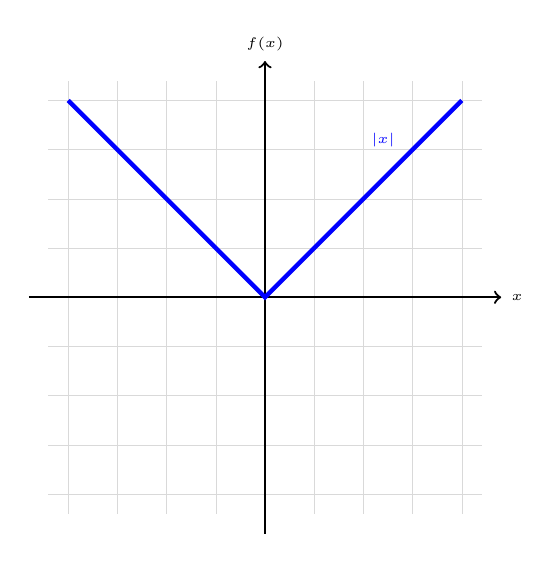
\begin{tikzpicture}[scale=2.5]
          % Square grid and axes
          \draw[help lines, color=gray!30, step=0.25cm] (-1.1,-1.1) grid (1.1,1.1);
          \draw[->, thick] (-1.2,0) -- (1.2,0) node[right] {\tiny $x$};
          \draw[->, thick] (0,-1.2) -- (0,1.2) node[above] {\tiny $f(x)$};
          
          % Plot
          \draw[ultra thick, blue] (-1,1) -- (0,0) -- (1,1);
          \node[blue, fill=white, inner sep=1pt] at (0.6,0.8) {\tiny $|x|$};
        \end{tikzpicture}
        \caption{$f(x) = |x|$}
      \end{subfigure}
      \hfill 
      \begin{subfigure}[b]{0.49\textwidth}
        \centering
        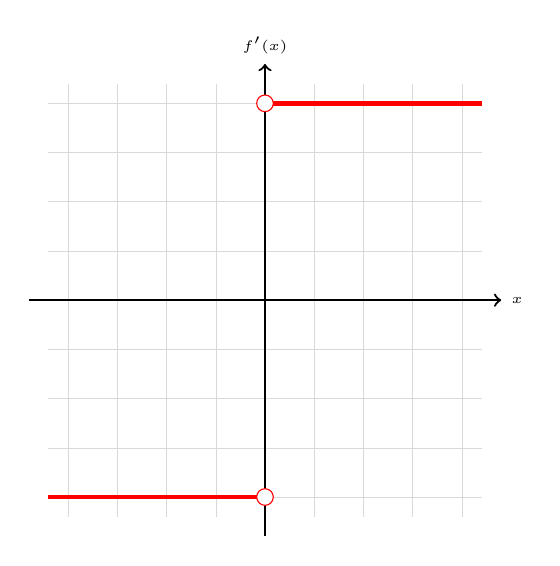
\begin{tikzpicture}[scale=2.5]
          \draw[help lines, color=gray!30, step=0.25cm] (-1.1,-1.1) grid (1.1,1.1);
          \draw[->, thick] (-1.2,0) -- (1.2,0) node[right] {\tiny $x$};
          \draw[->, thick] (0,-1.2) -- (0,1.2) node[above] {\tiny $f'(x)$};
          
          % Plot
          \draw[ultra thick, red] (-1.1,-1) -- (0,-1);
          \draw[ultra thick, red] (0,1) -- (1.1,1);
          \draw[red, fill=white] (0,-1) circle (1.2pt);
          \draw[red, fill=white] (0,1) circle (1.2pt);
        \end{tikzpicture}
        \caption{$f'(x) = \text{sgn}(x)$}
      \end{subfigure}
      \caption{The cusp at the origin in $f(x)$ corresponds to the jump discontinuity in $f'(x)$.}
    \end{figure}
  \end{example}

  \begin{example}[Differentiable but Not Continuously Differentiable]
    Consider the oscillatory function:
    \begin{equation}
        f(x) = \begin{cases} x^2 \sin\left(\frac{1}{x}\right) & x \neq 0 \\ 0 & x = 0 \end{cases}
    \end{equation}
    
    \begin{figure}[H]
      \centering
      \begin{subfigure}[b]{0.49\textwidth}
        \centering
        % Zoomed scale: increased to 5.0 for magnification
        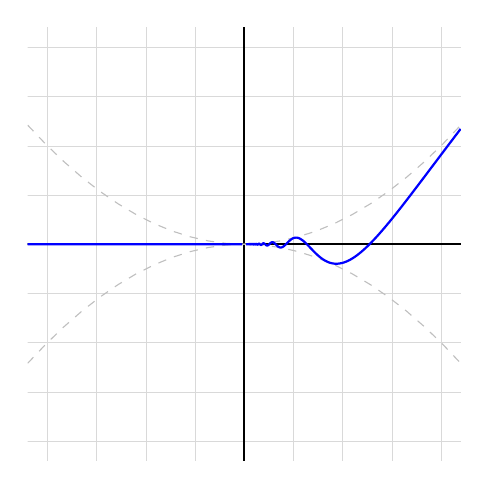
\begin{tikzpicture}[scale=5.0]
          \clip (-0.55,-0.55) rectangle (0.55,0.55);
          \draw[help lines, color=gray!30, step=0.125cm] (-0.6,-0.6) grid (0.6,0.6);
          \draw[->, thick] (-0.6,0) -- (0.6,0) node[right] {\tiny $x$};
          \draw[->, thick] (0,-0.6) -- (0,0.6) node[above] {\tiny $f(x)$};
          
          \draw[dashed, gray!50, domain=-0.55:0.55] plot (\x, {\x*\x});
          \draw[dashed, gray!50, domain=-0.55:0.55] plot (\x, {-\x*\x});
          
          \draw[thick, blue, domain=-0.55:-0.005, samples=1500] plot ({\x}, {\x*\x*sin(1/\x r)});
          \draw[thick, blue, domain=0.005:0.55, samples=1500] plot ({\x}, {\x*\x*sin(1/\x r)});
        \end{tikzpicture}
        \caption{$f(x)$ (Magnified at Origin)}
      \end{subfigure}
      \hfill 
      \begin{subfigure}[b]{0.49\textwidth}
        \centering
        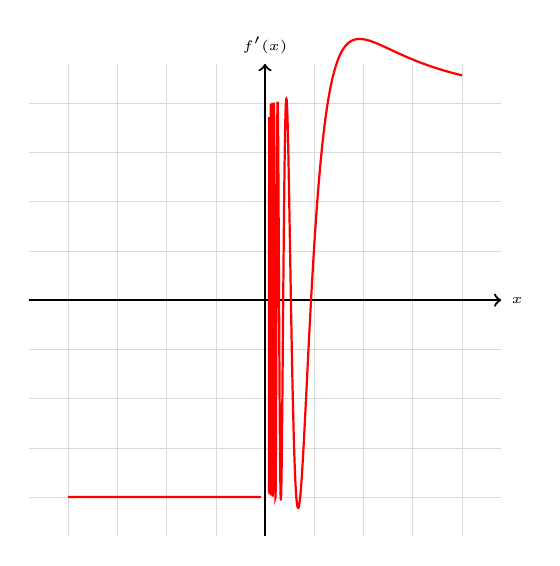
\begin{tikzpicture}[scale=2.5]
          \draw[help lines, color=gray!30, step=0.25cm] (-1.2,-1.2) grid (1.2,1.2);
          \draw[->, thick] (-1.2,0) -- (1.2,0) node[right] {\tiny $x$};
          \draw[->, thick] (0,-1.2) -- (0,1.2) node[above] {\tiny $f'(x)$};
          
          \draw[thick, red, domain=-1:-0.02, samples=1800] plot ({\x}, {2*\x*sin(1/\x r) - cos(1/\x r)});
          \draw[thick, red, domain=0.02:1, samples=1800] plot ({\x}, {2*\x*sin(1/\x r) - cos(1/\x r)});
        \end{tikzpicture}
        \caption{$f'(x)$ oscillation}
      \end{subfigure}
    \end{figure}
  \end{example}

  \begin{example}[Continuously Differentiable but No Second Derivative]
    Consider the signed square function:
    \begin{equation}
        f(x) = x|x|
    \end{equation}
    The derivative is $f'(x) = 2|x|$. While $f'$ is continuous ($C^0$), it is not differentiable at $x=0$, so $f$ is not $C^2$.

    \begin{figure}[H]
      \centering
      \begin{subfigure}[b]{0.49\textwidth}
        \centering
        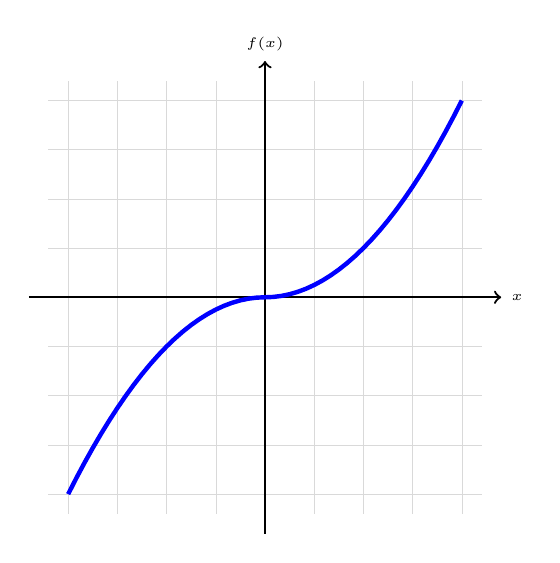
\begin{tikzpicture}[scale=2.5]
          % Square grid and axes
          \draw[help lines, color=gray!30, step=0.25cm] (-1.1,-1.1) grid (1.1,1.1);
          \draw[->, thick] (-1.2,0) -- (1.2,0) node[right] {\tiny $x$};
          \draw[->, thick] (0,-1.2) -- (0,1.2) node[above] {\tiny $f(x)$};
          
          % Plot
          \draw[ultra thick, blue, domain=0:1] plot ({\x}, {\x*\x});
          \draw[ultra thick, blue, domain=-1:0] plot ({\x}, {-\x*\x});
        \end{tikzpicture}
        \caption{$f(x) = x|x|$}
      \end{subfigure}
      \hfill 
      \begin{subfigure}[b]{0.49\textwidth}
        \centering
        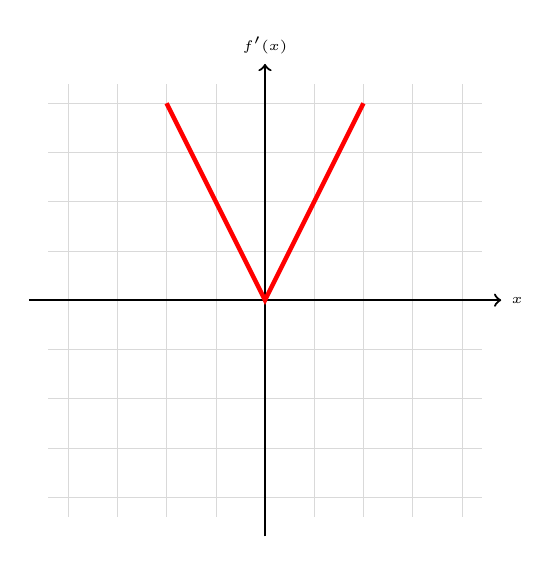
\begin{tikzpicture}[scale=2.5]
          \draw[help lines, color=gray!30, step=0.25cm] (-1.1,-1.1) grid (1.1,1.1);
          \draw[->, thick] (-1.2,0) -- (1.2,0) node[right] {\tiny $x$};
          \draw[->, thick] (0,-1.2) -- (0,1.2) node[above] {\tiny $f'(x)$};
          
          % Plot (derivative is 2|x|)
          \draw[ultra thick, red] (-0.5,1) -- (0,0) -- (0.5,1);
        \end{tikzpicture}
        \caption{$f'(x) = 2|x|$}
      \end{subfigure}
      \caption{A $C^1$ function has a continuous derivative, but that derivative may still have a cusp.}
    \end{figure}
  \end{example}
  
  \begin{theorem}[$C^1$ Implies Lipschitz]
    A continuously differentiable function is Lipschitz continuous. 
  \end{theorem}
  \begin{proof}
    
  \end{proof} 

  \begin{example}[Differentiable But Not Lipschitz]
    Consider 
    \begin{equation}
      f: (0, +\infty), f(x) = \sqrt{x}, \quad f^\prime (x) = \frac{1}{2 \sqrt{x}}
    \end{equation}
    Then, the derivative is unbounded around $0$. 
  \end{example}

  \begin{theorem}[L'Hopital's Rule]
    Suppose $f, g$ are continuously differentiable functions with $f(c) = g(c) = 0$ and $g^\prime (c) \neq 0$. Then, 
    \begin{equation}
      \lim_{x \to c} \frac{f(x)}{g(x)} = \lim_{x \to c} \frac{f^\prime (x)}{g^\prime (x)}
    \end{equation}
  \end{theorem}
  \begin{proof}
    We have 
    \begin{align}
      \lim_{x \to c} \frac{f(x)}{g(x)} & = \lim_{x \to c} \frac{f(x) - f(c)}{g(x) - g(c)} \\ 
                                       & = \lim_{x \to c} \frac{\frac{f(x) - f(c)}{x -  c}}{\frac{g(x) - g(c)}{x - c}} \\ 
                                       & = \frac{\lim_{x \to c} \frac{f(x) - f(c)}{x - c}}{\lim_{x \to c} \frac{g(x) - g(c)}{x - c}} \\ 
                                       & = \lim_{x \to c} \frac{f^\prime (x)}{g^\prime (x)}
    \end{align}
  \end{proof}

  \begin{example}[Limit of $sin(x)/x$]
    We can see that 
    \begin{equation}
      \lim_{x \to 0} \frac{\sin(x)}{x} = \lim_{x \to 0} \frac{\cos(x)}{1} = 1
    \end{equation}
  \end{example}

  \begin{example}
    Let $f(x) = \sin{x}$ and $g(x) = -0.5x$. Then, the function 
    \begin{equation}
      h(x) = \frac{f(x)}{g(x)} = \frac{\sin{x}}{-0.5x}
    \end{equation}
    is clearly undefined at $x = 0$. 
    However, we can solve the limit using L'Hopital's rule to get
    \begin{equation}
      \lim_{x \rightarrow 0} \frac{\sin{x}}{-0.5x} = \lim_{x \rightarrow 0} \frac{\cos{x}}{-0.5} = -2
    \end{equation}
    Therefore, $h: \mathbb{R} \setminus 0 \longrightarrow \mathbb{R}$ can be completed to continuous function on all of $\mathbb{R}$ by defining the extension: 
    \begin{equation}
      H(x) \coloneqq \begin{cases} h(x), & x \neq 0 \\ -2, & x = 0 \end{cases} 
    \end{equation}
  \end{example}

\subsection{Taylor's Formula} 

  Taylor's formula is quite misunderstood when you first learn about it, and most people don't know that there are two separate theorems on it with two completely different purposes. The first one from Lagrange extends the MVT and the purpose is to find an explicit formula for the error value. The second from Peano extends the definition of differentiability to higher order terms, and the main purpose is to tell you how fast the error term vanishes. Their assumptions are also completely different, too. 

  Let's start with Peano's first. So far, we have constructed a linear approximation, but let's step back for a moment and try to construct successive approximations to an arbitrary function $f: E \longrightarrow \mathbb{R}$ around a given point $x_0$. That is, we find a function $g$ such that
  \begin{equation}
    f(x) = g(x) + o(g)
  \end{equation}
  Depending on what $g$ is, we can construct better approximations of $f$. 
  \begin{enumerate}
    \item \textit{Constant Approximation}. The 0th order approximation is when $g$ is a constant. So 
      \begin{equation}
        f(x) = c_0 + o(1) \text{ as } x \to x_0
      \end{equation}
      which basically means that we want the difference $f(x) - c_0 \in o(1)$. If $f$ is continuous\footnote{This is important!}, the only possible case is when $c_0 = f(x)$.  

    \item \textit{Linear Approximation}. We have already done the 1st order approximation, since we just set 
      \begin{equation}
        f(x) = c_0 + c_1 (x - x_0) + o(x - x_0) \text{ as } x \to x_0
      \end{equation}
      If we assume $f$ is continuous, then we must have $c_0 = f(x)$ since $c_1 (x - x_0)$ will vanish. Then, we have already proven that $c_1 = f^{\prime} (x_0)$. 

    \item \textit{Quadratic Approximation}. We can continue this pattern to try and find a quadratic approximation of $f$ in the form
      \begin{equation}
        f(x) = c_0 + c_1 (x - x_0) + c_2 (x - x_0)^2 + o\big((x - x_0)^2 \big) \text{ as } x \rightarrow x_0
      \end{equation}
      By assuming continuity of $f$, we can derive $c_0 = f(x_0)$. Furthermore, continuity of the derivative will imply $c_1 = f^\prime (x_0)$. What should our guess be for $c_2$? Well, we can rearrange the terms so that 
      \begin{align}
        c_2 & = \frac{f(x) - c_0 - c_1 (x - x_0) - o ((x - x_0)^2 )}{(x - x_0)^2} \\ 
            & = \frac{f(x) - c_0 - c_1 (x - x_0)}{(x - x_0)^2} - o(1) 
      \end{align}
      Now for such polynomial coefficients to exist, $c_2$ must be constant, so the right hand ride shouldn't depend on $x$. We can take advantage of the $o(1)$ term by setting the limit $x \to x_0$. By using L'Hopital's rule, we have 
      \begin{equation}
        c_2 = \lim_{x \to x_0} \frac{f(x) - c_0 - c_1 (x - x_0)}{(x - x_0)^2} = \lim_{x \to x_0} \frac{f^\prime (x) - c_1}{2 (x - x_0)} = \frac{1}{2} f^{\prime\prime} (x_0)
      \end{equation}

      We then postulate that $c_2 = \frac{1}{2} f^{\prime\prime} (x_0)$ and define the error term as 
      \begin{equation}
        \varphi(x) = f(x) - f(x_0) - f^\prime (x_0) (x - x_0) - \frac{f^{\prime\prime} (x_0)}{2} (x - x_0)^2 
      \end{equation}
      We claim that it is $o((x - x_0)^2)$. Indeed, using L'Hopital's rule
      \begin{align}
        \lim_{x \to x_0} \frac{\varphi(x)}{(x - x_0)^2} & = \lim_{x \to x_0} \bigg( \frac{f(x) - f(x_0) - f^\prime (x_0) (x - x_0)}{(x - x_0)^2} - \frac{f^{\prime\prime}(x_0)}{2}\bigg) \\
                                                        & = \lim_{x \to x_0} \bigg( \frac{f^\prime(x) - f^\prime (x_0)}{2 (x - x_0)} \bigg) - \frac{f^{\prime\prime} (x_0)}{2} \\ 
                                                        & = \frac{f^{\prime\prime} (x_0)}{2} - \frac{f^{\prime\prime} (x_0)}{2} = 0 
      \end{align}
      and we are done. 
  \end{enumerate}

  At this point, the pattern is pretty clear. 

  \begin{theorem}[Taylor's Theorem with Peano's Form of Remainder]
    If $f: [a, b] \to \mathbb{R}$ is $n$-times differentiable at point $x_0 \in (a, b)$, then there exists an $o \big( (x - x_0)^n \big)$  function such that 
    \begin{equation}
      f(x) = \bigg( \sum_{k=0}^n \frac{f^{(k)}(x_0)}{k!} (x - x_0)^k  \bigg) + o \big( (x - x_0)^n \big)
    \end{equation} 
  \end{theorem}
  \begin{proof}
    We prove by induction. The cases for $n = 0, 1, 2$ are done above. Now assume that this holds for $n-1$. We are seeking a polynomial $P_n(x; x_0) = c_0 + c_1 (x - x_0) + \ldots + c_n (x - x_0)^n$ such that
    \begin{equation}
      f(x) = c_0 + c_1 (x - x_0) + \ldots + c_n (x - x_0)^n + o\big((x - x_0)^n\big) \text{ as } x \rightarrow x_0
    \end{equation}
    Since $c_n (x - x_0)^n \in o((x - x_0)^{n-1})$, we also know that $c_n (x - x_0)^n + o ((x - x_0)^n ) \in o((x - x_0)^{n-1})$, and so such a polynomial must also satisfy 
    \begin{equation}
      f(x) = c_0 + c_1 (x - x_0) + \ldots + c_{n-1} (x - x_0)^{n-1} + o\big((x - x_0)^{n-1}\big) \text{ as } x \rightarrow x_0
    \end{equation}
    Since any solution $c_0, \ldots, c_n$ must satisfy the above for $c_0, \ldots, c_{n-1}$, we can invoke our induction step for $n-1$ to see that 
    \begin{equation}
      c_k = \frac{f^{(k)} (x_0)}{k!} (x - x_0)^k, \qquad k = 0, 1, \ldots, n-1
    \end{equation}
    To make a guess for $c_n$, we do some algebra to isolate 
    \begin{align}
      c_n & = \frac{f(x) - \big(c_0 + c_1 (x - x_0) + \ldots + c_{n-1} (x - x_0)^{n-1} + o ((x - x_0)^{n}) \big)}{(x - x_0)^n} \\  
          & = \frac{f(x) - \big(c_0 + c_1 (x - x_0) + \ldots + c_{n-1} (x - x_0)^{n-1} \big)}{(x - x_0)^{n}} - o(1) \\  
    \end{align}
    and by taking the limit, with repeated application of L'Hopital's rule $n-1$ times, 
    \begin{equation}
      c_n = \lim_{x \rightarrow x_0} \frac{f(x) - (c_0 + \ldots + c_{n-1}(x - x_0)^{n-1})}{(x - x_0)^n} = \lim_{x \to x_0} \frac{f^{(n-1)} (x) - f^{(n-1)} (x_0)}{n! (x - x_0)} = \frac{1}{n!} f^{(n)} (x_0)
    \end{equation}
    Now we claim that $c_n = \frac{1}{n!} f^{(n)} (x_0)$, and all that's left to do is show that the error term 
    \begin{equation}
      \varphi(x) = f(x) - \sum_{k=0}^{n} \frac{f^{(k)} (x_0)}{k!} (x - x_0)^k \in o \big( (x - x_0)^{n-1} \big)
    \end{equation}
    Indeed, we have 
    \begin{align}
      \lim_{x \to x_0} \frac{\varphi(x)}{(x - x_0)^n} & = \lim_{x \to x_0} \frac{f(x) - f(x_0) - f^\prime (x_0) (x - x_0) - \frac{1}{2} f^{\prime\prime} (x_0) (x - x_0)^2 - \ldots - \frac{1}{n!} f^{(n)} (x_0) (x - x_0)^n}{(x - x_0)^n}  \\ 
                                                      & = \lim_{x \to x_0} \frac{f(x) - f(x_0) - \ldots - \frac{1}{(n-1)!} f^{(n-1)} (x_0) (x - x_0)^{n-1}}{(x - x_0)^n} - \frac{1}{n!} f^{(n)} (x_0) \\ 
                                                      & = \lim_{x \to x_0} \frac{f^{(n-1)} (x) - f^{(n-1)} (x_0)}{n! (x - x_0)} - \frac{1}{n!} f^{(n)} (x_0) \\ 
                                                      & = \frac{1}{n!} f^{(n)} (x_0) - \frac{1}{n!} f^{(n)} (x_0) = 0
    \end{align}
  \end{proof}

  Given differentiable $f: [a, b] \to \mathbb{R}$, and $x_0 \in [a, b]$, say that we want to try and approximate $f(x)$ with $f(x_0)$. Using MVT on the closed subinterval $[x_0, x]$\footnote{or $[x, x_0]$ if $x < x_0$}, we can find a $c \in (x_0, x)$ s.t. $f(x) = f(x_0) + f^\prime (c) (x - x_0)$. This is like a first order approximation, and perhaps we can extend this if we have an additional assumption that $f$ is twice differentiable. To do this, recall how we proved the MVT. We subtracted a linear function from $f(x)$ to get a new function $g(x)$ satisfying $g(a) = g(b) = 0$. Now we can perform this again to get higher order approximations. 

  \begin{lemma}[Taylor's Formula of Order 2 with Lagrange's Form of Remainder]
    Suppose $f: [a, b] \to \mathbb{R}$
    \begin{enumerate}
      \item is twice differentiable over $(a, b)$, and 
      \item is $C^1$ over $[a, b]$. 
    \end{enumerate}
    Then, there exists a $\xi$ between $x_0$ and $x$ s.t. 
    \begin{equation}
      f(x) = f(x_0) + f^\prime (x_0) (x - x_0) + \frac{f^{\prime \prime}(\xi)}{2} (x - x_0)^2
    \end{equation} 
  \end{lemma}
  \begin{proof}
    Let us define the function 
    \begin{equation}
      g(x) \coloneqq f(x) - f(a) - f^\prime (a) (x - a) - M (x - a)^2
    \end{equation} 

    where $M$ was chosen such that $g(b) = 0$. Now notice that 
    \begin{align}
      g(a) & = f(a) - f(a) - 0 - 0 = 0 \\ 
      g^\prime (a) & = f^\prime (a) - f^\prime (a) - 0 = 0 
    \end{align}

    and so by using Rolle's theorem on $g$, there exists a $c_1 \in (a, b)$ s.t. 
    \begin{equation}
      g^\prime (c_1) (b - a) = g(b) - g(a) = 0 - 0 = 0 \implies g^\prime (c_1) = 0
    \end{equation}  

    therefore, we can use Rolle's theorem again on $g^\prime$ and claim there exists a $c \in (a, c_1)$ s.t. 
    \begin{equation}
      g^{\prime\prime} (c) (c_1 - a) = g^\prime (c_1) - g^\prime (a) = 0 - 0 = 0 \implies g^{\prime\prime} (c) = 0
    \end{equation}

    This gives us all we need. By taking the double derivative of $g$, we get 
    \begin{equation}
      0 = g^{\prime\prime} (c) = f^{\prime\prime} (c) - 2M \implies M = \frac{f^{\prime\prime} (c)}{2}
    \end{equation}

    and substituting this in gives 
    \begin{equation}
      0 = g(b) = f(b) - f(a) - f^\prime (a) (b - a) - \frac{f^{\prime\prime} (c)}{2} (b - a)^2
    \end{equation}
  \end{proof}

  This is like a mean value theorem for the second order, where only the final term is dependent on $c$. We can continue this process to get a $n$th order approximation. 

  \begin{theorem}[Taylor's Theorem with Lagrange's Form of Remainder]
    Suppose $f: [a, b] \to \mathbb{R}$
    \begin{enumerate}
      \item is $(n+1)$-times differentiable over $(a, b)$, and 
      \item is $C^{n}$ over $[a, b]$. 
    \end{enumerate}
    Then, there exists a $\xi$ between $x_0$ and $x$ s.t. 
    \begin{equation}
      f(x) = \bigg( \sum_{k=0}^n \frac{f^{(k)}(x_0)}{k!} (x - x_0)^k  \bigg) + \frac{f^{(n+1)} (\xi)}{(n+1)!} (x - x_0)^{n+1}
    \end{equation} 
  \end{theorem}
  \begin{proof}
    We do the exact same process. Let us define 
    \begin{equation}
      P(x) = \sum_{k=0}^n \frac{f^{(k)} (a)}{k!} (x - a)^k
    \end{equation} 
    and set 
    \begin{equation}
      g(x) \coloneqq f(x) - P(x) - M (x - a)^{n+1}
    \end{equation} 
    where $M$ was chosen such that $g(b) = 0$. Now notice that evaluating on $g$ gives us 
    \begin{equation}
      g(a) = g^\prime (a) = g^{\prime\prime} (a) = \ldots = g^{(n)} (a) = 0 
    \end{equation} 
    So by using Rolle's theorem on $g$, there exists a $c_1 \in (a, b)$ s.t. $g^\prime (c_1) = 0$. Therefore we can use Rolle's theorem on $g^\prime$ to show there exists a $c_2 \in (a, c_1)$. We keep doing this until we show that there exists a $c \in (a, b)$ s.t. $g^{(n)} (c) = 0$. With this, we can directly evaluating the $n$th derivative of $g$ to find 
    \begin{equation}
      0 = g^{(n)} (c) = f^{(n)} (c) - n! M \implies M = \frac{f^{(n)} (c)}{n!}
    \end{equation}
  \end{proof}

\subsection{Extrema and Concavity}

  Similarly, we can connect the concepts of extrema and derivatives. 

  \begin{theorem}[First Derivative Test]
    Let $f: [a, b] \to \mathbb{R}$ and assume $f$ has a local maximum at $c \in (a, b)$ with $f$ differentiable at $c$. Then $f^\prime (c) = 0$. 
  \end{theorem}
  \begin{proof}
    Let us pick two sequences---a left one and a right one---that converges to $x$ from either side. 
    \begin{enumerate}
      \item If $x > c$ (with $x$ sufficiently close to $c$), then $f(c) \geq f(x)$ and so 
      \begin{equation}
        \frac{f(c) - f(x)}{c - x} \leq 0 \implies f^\prime (c) = \lim_{c - x} \frac{f(c) - f(x)}{c - x} \leq 0
      \end{equation}

      \item If $x < c$, then $f(c) \geq f(x)$ and so 
      \begin{equation}
        \frac{f(c) - f(x)}{c - x} \geq 0 \implies f^\prime (c) = \lim_{c - x} \frac{f(c) - f(x)}{c - x} \geq 0
      \end{equation}
    \end{enumerate}
    So $0 \leq f^\prime (c) \leq 0 \implies f^\prime(c) = 0$. 
  \end{proof}

  \begin{definition}[Convex, Concave Functions]
    A function $f: (a, b) \longrightarrow \mathbb{R}$ defined on an open interval $(a, b) \subset \mathbb{R}$ is \textbf{convex} if the inequality
    \begin{equation}
      f( \alpha_1 x_1 + \alpha_2 x_2) \leq \alpha_1 f(x_1) + \alpha_2 f(x_2)
    \end{equation}
    holds and \textbf{concave}, or \textbf{convex upward}, if the inequality 
    \begin{equation}
      f( \alpha_1 x_1 + \alpha_2 x_2) \geq \alpha_1 f(x_1) + \alpha_2 f(x_2)
    \end{equation}
    holds for all pairs of points $x_1, x_2 \in (a, b)$ and any numbers $\alpha_1, \alpha_2 \geq 0$ such that $\alpha_1 + \alpha_2 = 1$. If this inequality is strict whenever $x_1 \neq x_2$ and $\alpha_1 \alpha_2 \neq 0$, the function is said to be \textbf{strictly convex} and \textbf{strictly concave}, respectively. 
  \end{definition}

  Note that using induction on the number of points, we get a primitive form of Jensen's inequality. 

  \begin{lemma}[Jensen's Inequality]
    If $f: (a, b) \longrightarrow \mathbb{R}$ is a convex function, $x_1, ..., x_n$ are points of $(a, b)$, and $\alpha_1, ..., \alpha_n$ are nonnegative numbers such that $\alpha_1 + ... + \alpha_n = 1$, then 
    \begin{equation}
      f(\alpha_1 x_1 + ... + \alpha_n x_n) \leq \alpha_1 f(x_1) + ... + \alpha_n f(x_n)
    \end{equation}
  \end{lemma}

  The following is also another equivalent condition for a function to be convex over $(a, b)$. 

  \begin{theorem}
    A function $f: (a, b) \longrightarrow \mathbb{R}$ that is differentiable on the open interval $(a, b)$ is convex on $(a, b)$ if and only if its graph contains no points below any tangent drawn to it.
  \end{theorem}

  \begin{theorem}[2nd Derivatives of Convex Functions]
    Given a function $f: (a, b) \longrightarrow \mathbb{R}$ that is differentiable in its domain, 
    \begin{enumerate}
      \item $f$ is convex $\iff f^\prime$ is increasing on $(a, b) \iff f^{\prime\prime} \geq 0$ on $(a, b)$ 
      \item $f$ is strictly convex $\iff f^\prime$ is strictly increasing on $(a, b) \iff f^{\prime\prime} > 0$ on $(a, b)$ 
      \item $f$ is concave $\iff f^\prime$ is decreasing on $(a, b) \iff f^{\prime\prime} \leq 0$ on $(a, b)$ 
      \item $f$ is strictly concave $\iff f^\prime$ is strictly decreasing on $(a, b) \iff f^{\prime\prime} < 0$ on $(a, b)$ 
    \end{enumerate}
  \end{theorem}

  \begin{definition}[Inflection Point]
    Let $f: E \longrightarrow \mathbb{R}$ be a function defined and differentiable on a neighborhood $U(x_0)$. If the function is convex downward (resp. upward) on the set $\mathring{U}^- (x_0) = \{x \in U(x_0) \;|\; x < x_0\}$ and convex upward (resp. downward) on $\mathring{U}^+ (x_0) = \{x \in U(x_0)\;|\; x > x_0\}$, then the point 
    \begin{equation}
      \big( x_0, f(x_0) \big)
    \end{equation}
    is called a \textbf{inflection point of the graph}. 

    \begin{figure}[H]
      \centering 
      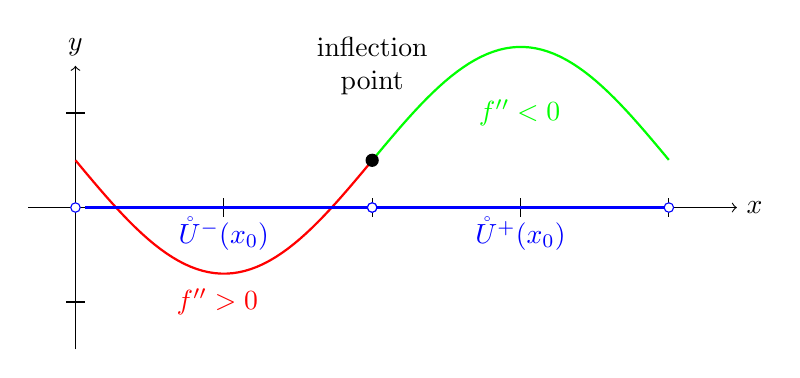
\begin{tikzpicture}[scale=1.2]
        % Draw coordinate axes
        \draw[->] (-0.5,0) -- (7,0) node[right] {$x$};
        \draw[->] (0,-1.5) -- (0,1.5) node[above] {$y$};
        
        % Draw the negative sine curve in two colors, shifted up by 0.5
        \draw[thick, red] plot[domain=0:3.14, samples=50] (\x, {-sin(\x r) * 1.2 + 0.5});
        \draw[thick, green] plot[domain=3.14:6.28, samples=50] (\x, {-sin(\x r) * 1.2 + 0.5});
        
        % Add second derivative labels
        \node[red] at (1.5,-1) {$f^{\prime\prime} > 0$};
        \node[green] at (4.7,1) {$f^{\prime\prime} < 0$};
        
        % Add inflection point label - updated y-coordinate to match the shift
        \fill (3.14,0.5) circle (0.07);
        \node[align=center] at (3.14,1.5) {inflection\\point};
        
        % Add key points on x-axis (ticks only, no labels)
        \foreach \x in {0, 1.57, 3.14, 4.71, 6.28} {
          \draw (\x,0.1) -- (\x,-0.1);
        }
        
        % Add blue intervals with hollow endpoints
        % First interval (0, pi)
        \draw[blue, thick] (0.1,0) -- (3.14,0);
        \draw[blue, fill=white] (0.0,0) circle (0.05);
        \draw[blue, fill=white] (3.14,0) circle (0.05);
        \node[blue, below] at (1.57,0) {$\mathring{U}^{-}(x_0)$};
        
        % Second interval (pi, 2pi)
        \draw[blue, thick] (3.14,0) -- (6.28,0);
        \draw[blue, fill=white] (3.14,0) circle (0.05);
        \draw[blue, fill=white] (6.28,0) circle (0.05);
        \node[blue, below] at (4.71,0) {$\mathring{U}^{+}(x_0)$};
        
        % Add key points on y-axis (ticks only, no labels)
        \foreach \y in {-1, 1} {
          \draw (0.1,\y) -- (-0.1,\y);
        }
      \end{tikzpicture}
      \caption{Curve with changing concavity and inflection point at $\pi$}
      \label{fig:neg-sine-concavity}
    \end{figure}
  \end{definition}

\subsection{Exercises}

  \begin{exercise}[Rudin 5.1]
    Let $f$ be defined for all real $x$, and suppose that
    \begin{equation}
      |f(x) - f(y)| \le (x - y)^2
    \end{equation}
    for all real $x$ and $y$. Prove that $f$ is constant.
  \end{exercise}
  \begin{solution}

  \end{solution}

  \begin{exercise}[Rudin 5.2]
    Suppose $f^\prime(x) > 0$ in $(a, b)$. Prove that $f$ is strictly increasing in $(a, b)$, and let $g$ be its inverse function. Prove that $g$ is differentiable, and that
    \begin{equation}
      g^\prime(f(x)) = \frac{1}{f^\prime(x)} \quad (a < x < b)
    \end{equation}
   .
  \end{exercise}
  \begin{solution}

  \end{solution}

  \begin{exercise}[Rudin 5.3]
    Suppose $g$ is a real function on $R^1$, with bounded derivative (say $|g^\prime| \le M$). Fix $\epsilon > 0$, and define $f(x) = x + \epsilon g(x)$. Prove that $f$ is one-to-one if $\epsilon$ is small enough. (A set of admissible values of $\epsilon$ can be determined which depends only on $M$.)
  \end{exercise}
  \begin{solution}

  \end{solution}

  \begin{exercise}[Rudin 5.4]
    If
    \begin{equation}
      C_0 + \frac{C_1}{2} + \dots + \frac{C_{n-1}}{n} + \frac{C_n}{n+1} = 0
    \end{equation}
    where $C_0, \dots, C_n$ are real constants, prove that the equation
    \begin{equation}
      C_0 + C_1 x + \dots + C_{n-1} x^{n-1} + C_n x^n = 0
    \end{equation}
    has at least one real root between 0 and 1.
  \end{exercise}
  \begin{solution}

  \end{solution}

  \begin{exercise}[Rudin 5.5]
    Suppose $f$ is defined and differentiable for every $x > 0$, and $f^\prime(x) \to 0$ as $x \to +\infty$. Put $g(x) = f(x + 1) - f(x)$. Prove that $g(x) \to 0$ as $x \to +\infty$.
  \end{exercise}
  \begin{solution}

  \end{solution}

  \begin{exercise}[Rudin 5.6]
    Suppose
    \begin{enumerate}
      \item[(a)] $f$ is continuous for $x \ge 0$,
      \item[(b)] $f^\prime(x)$ exists for $x > 0$,
      \item[(c)] $f(0) = 0$,
      \item[(d)] $f^\prime$ is monotonically increasing.
    \end{enumerate}
    Put
    \begin{equation}
      g(x) = \frac{f(x)}{x} \quad (x > 0)
    \end{equation}
    and prove that $g$ is monotonically increasing.
  \end{exercise}
  \begin{solution}

  \end{solution}

  \begin{exercise}[Rudin 5.7]
    Suppose $f^\prime(x), g^\prime(x)$ exist, $g^\prime(x) \ne 0$, and $f(x) = g(x) = 0$. Prove that
    \begin{equation}
      \lim_{t \to x} \frac{f(t)}{g(t)} = \frac{f^\prime(x)}{g^\prime(x)}
    \end{equation}
   . (This holds also for complex functions.)
  \end{exercise}
  \begin{solution}

  \end{solution}

  \begin{exercise}[Rudin 5.8]
    Suppose $f^\prime$ is continuous on $[a, b]$ and $\epsilon > 0$. Prove that there exists $\delta > 0$ such that
    \begin{equation}
      \left| \frac{f(t) - f(x)}{t - x} - f^\prime(x) \right| < \epsilon
    \end{equation}
    whenever $0 < |t - x| < \delta, a \le x \le b, a \le t \le b$. (This could be expressed by saying that $f$ is uniformly differentiable on $[a, b]$ if $f^\prime$ is continuous on $[a, b]$.) Does this hold for vector-valued functions too?
  \end{exercise}
  \begin{solution}

  \end{solution}

  \begin{exercise}[Rudin 5.9]
    Let $f$ be a continuous real function on $R^1$, of which it is known that $f^\prime(x)$ exists for all $x \ne 0$ and that $f^\prime(x) \to 3$ as $x \to 0$. Does it follow that $f^\prime(0)$ exists?
  \end{exercise}
  \begin{solution}

  \end{solution}

  \begin{exercise}[Rudin 5.10]
    Suppose $f$ and $g$ are complex differentiable functions on $(0, 1)$, $f(x) \to 0, g(x) \to 0, f^\prime(x) \to A, g^\prime(x) \to B$ as $x \to 0$, where $A$ and $B$ are complex numbers, $B \ne 0$. Prove that
    \begin{equation}
      \lim_{x \to 0} \frac{f(x)}{g(x)} = \frac{A}{B}
    \end{equation}
   . Compare with Example 5.18. \textit{Hint:}
    \begin{equation}
      \frac{f(x)}{g(x)} = \left\{ \frac{f(x)}{x} - A \right\} \cdot \frac{x}{g(x)} + A \cdot \frac{x}{g(x)}
    \end{equation}
   . Apply Theorem 5.13 to the real and imaginary parts of $f(x)/x$ and $g(x)/x$.
  \end{exercise}
  \begin{solution}

  \end{solution}

  \begin{exercise}[Rudin 5.11]
    Suppose $f$ is defined in a neighborhood of $x$, and suppose $f^{\prime\prime}(x)$ exists. Show that
    \begin{equation}
      \lim_{h \to 0} \frac{f(x + h) + f(x - h) - 2f(x)}{h^2} = f^{\prime\prime}(x)
    \end{equation}
   . Show by an example that the limit may exist even if $f^{\prime\prime}(x)$ does not. \textit{Hint:} Use Theorem 5.13.
  \end{exercise}
  \begin{solution}

  \end{solution}

  \begin{exercise}[Rudin 5.12]
    If $f(x) = |x|^3$, compute $f^\prime(x), f^{\prime\prime}(x)$ for all real $x$, and show that $f^{(3)}(0)$ does not exist.
  \end{exercise}
  \begin{solution}

  \end{solution}

  \begin{exercise}[Rudin 5.13]
    Suppose $a$ and $c$ are real numbers, $c > 0$, and $f$ is defined on $[-1, 1]$ by
    \begin{equation}
      f(x) = 
      \begin{cases}
        x^a \sin(|x|^{-c}) & (\text{if } x \ne 0), \\
        0 & (\text{if } x = 0)
      \end{cases}
    \end{equation}
   . Prove the following statements:
    \begin{enumerate}
      \item[(a)] $f$ is continuous if and only if $a > 0$.
      \item[(b)] $f^\prime(0)$ exists if and only if $a > 1$.
      \item[(c)] $f^\prime$ is bounded if and only if $a \ge 1 + c$.
      \item[(d)] $f^\prime$ is continuous if and only if $a > 1 + c$.
      \item[(e)] $f^{\prime\prime}(0)$ exists if and only if $a > 2 + c$.
      \item[(f)] $f^{\prime\prime}$ is bounded if and only if $a \ge 2 + 2c$.
      \item[(g)] $f^{\prime\prime}$ is continuous if and only if $a > 2 + 2c$.
    \end{enumerate}
  \end{exercise}
  \begin{solution}

  \end{solution}

  \begin{exercise}[Rudin 5.14]
    Let $f$ be a differentiable real function defined in $(a, b)$. Prove that $f$ is convex if and only if $f^\prime$ is monotonically increasing. Assume next that $f^{\prime\prime}(x)$ exists for every $x \in (a, b)$, and prove that $f$ is convex if and only if $f^{\prime\prime}(x) \ge 0$ for all $x \in (a, b)$.
  \end{exercise}
  \begin{solution}

  \end{solution}

  \begin{exercise}[Rudin 5.15]
    Suppose $a \in R^1$, $f$ is a twice-differentiable real function on $(a, \infty)$, and $M_0, M_1, M_2$ are the least upper bounds of $|f(x)|, |f^\prime(x)|, |f^{\prime\prime}(x)|$, respectively, on $(a, \infty)$. Prove that
    \begin{equation}
      M_1^2 \le 4M_0 M_2
    \end{equation}
   . \textit{Hint:} If $h > 0$, Taylor's theorem shows that
    \begin{equation}
      f^\prime(x) = \frac{1}{2h} [f(x + 2h) - f(x)] - hf^{\prime\prime}(\xi)
    \end{equation}
    for some $\xi \in (x, x + 2h)$. Hence
    \begin{equation}
      |f^\prime(x)| \le hM_2 + \frac{M_0}{h}
    \end{equation}
   . To show that $M_1^2 = 4M_0 M_2$ can actually happen, take $a = -1$, define
    \begin{equation}
      f(x) = 
      \begin{cases}
        2x^2 - 1 & (-1 < x < 0), \\
        \frac{x^2 - 1}{x^2 + 1} & (0 \le x < \infty)
      \end{cases}
    \end{equation}
    and show that $M_0 = 1, M_1 = 4, M_2 = 4$. Does $M_1^2 \le 4M_0 M_2$ hold for vector-valued functions too?
  \end{exercise}
  \begin{solution}

  \end{solution}

  \begin{exercise}[Rudin 5.16]
    Suppose $f$ is twice-differentiable on $(0, \infty)$, $f^{\prime\prime}$ is bounded on $(0, \infty)$, and $f(x) \to 0$ as $x \to \infty$. Prove that $f^\prime(x) \to 0$ as $x \to \infty$. \textit{Hint:} Let $a \to \infty$ in Exercise 15.
  \end{exercise}
  \begin{solution}

  \end{solution}

  \begin{exercise}[Rudin 5.17]
    Suppose $f$ is a real, three times differentiable function on $[-1, 1]$, such that
    \begin{equation}
      f(-1) = 0, \quad f(0) = 0, \quad f(1) = 1, \quad f^\prime(0) = 0
    \end{equation}
   . Prove that $f^{(3)}(x) \ge 3$ for some $x \in (-1, 1)$. Note that equality holds for $\frac{1}{2}(x^3 + x^2)$. \textit{Hint:} Use Theorem 5.15, with $\alpha = 0$ and $\beta = \pm 1$, to show that there exist $s \in (0, 1)$ and $t \in (-1, 0)$ such that $f^{(3)}(s) + f^{(3)}(t) = 6$.
  \end{exercise}
  \begin{solution}

  \end{solution}

  \begin{exercise}[Rudin 5.18]
    Suppose $f$ is a real function on $[a, b]$, $n$ is a positive integer, and $f^{(n-1)}$ exists for every $t \in [a, b]$. Let $\alpha, \beta$, and $P$ be as in Taylor's theorem (5.15). Define
    \begin{equation}
      Q(t) = \frac{f(t) - f(\beta)}{t - \beta}
    \end{equation}
    for $t \in [a, b], t \ne \beta$, differentiate $f(t) - f(\beta) = (t - \beta)Q(t)$ $n-1$ times at $t = \alpha$, and derive the following version of Taylor's theorem:
    \begin{equation}
      f(\beta) = P(\beta) + \frac{Q^{(n-1)}(\alpha)}{(n-1)!} (\beta - \alpha)^n
    \end{equation}
   .
  \end{exercise}
  \begin{solution}

  \end{solution}

  \begin{exercise}[Rudin 5.19]
    Suppose $f$ is defined in $(-1, 1)$ and $f^\prime(0)$ exists. Suppose $-1 < \alpha_n < \beta_n < 1$, $\alpha_n \to 0$, and $\beta_n \to 0$ as $n \to \infty$. Define the difference quotients
    \begin{equation}
      D_n = \frac{f(\beta_n) - f(\alpha_n)}{\beta_n - \alpha_n}
    \end{equation}
   . Prove the following statements:
    \begin{enumerate}
      \item[(a)] If $\alpha_n < 0 < \beta_n$, then $\lim D_n = f^\prime(0)$.
      \item[(b)] If $0 < \alpha_n < \beta_n$ and $\{\beta_n/(\beta_n - \alpha_n)\}$ is bounded, then $\lim D_n = f^\prime(0)$.
      \item[(c)] If $f^\prime$ is continuous in $(-1, 1)$, then $\lim D_n = f^\prime(0)$.
    \end{enumerate}
    Give an example in which $f$ is differentiable in $(-1, 1)$ (but $f^\prime$ is not continuous at 0) and in which $\alpha_n, \beta_n$ tend to 0 in such a way that $\lim D_n$ exists but is different from $f^\prime(0)$.
  \end{exercise}
  \begin{solution}

  \end{solution}

  \begin{exercise}[Rudin 5.22]
    Suppose $f$ is a real function on $(-\infty, \infty)$. Call $x$ a \textit{fixed point} of $f$ if $f(x) = x$.
    \begin{enumerate}
      \item[(a)] If $f$ is differentiable and $f^\prime(t) \ne 1$ for every real $t$, prove that $f$ has at most one fixed point.
      \item[(b)] Show that the function $f$ defined by
        \begin{equation}
          f(t) = t + (1 + e^t)^{-1}
        \end{equation}
        has no fixed point, although $0 < f^\prime(t) < 1$ for all real $t$.
      \item[(c)] However, if there is a constant $A < 1$ such that $|f^\prime(t)| \le A$ for all real $t$, prove that a fixed point $x$ of $f$ exists, and that $x = \lim x_n$, where $x_1$ is an arbitrary real number and $x_{n+1} = f(x_n)$ for $n = 1, 2, 3, \dots$.
      \item[(d)] Show that the process described in (c) can be visualized by the zig-zag path $(x_1, x_2) \to (x_2, x_2) \to (x_2, x_3) \to (x_3, x_3) \to (x_3, x_4) \to \dots$. 
    \end{enumerate}
  \end{exercise}
  \begin{solution}

  \end{solution}

  \begin{exercise}[Rudin 5.23]
    The function $f$ defined by
    \begin{equation}
      f(x) = \frac{x^3 + 1}{3}
    \end{equation}
    has three fixed points, say $\alpha, \beta, \gamma$, where
    \begin{equation}
      -2 < \alpha < -1, \quad 0 < \beta < 1, \quad 1 < \gamma < 2
    \end{equation}
   . For arbitrarily chosen $x_1$, define $\{x_n\}$ by setting $x_{n+1} = f(x_n)$.
    \begin{enumerate}
      \item[(a)] If $x_1 < \alpha$, prove that $x_n \to -\infty$ as $n \to \infty$.
      \item[(b)] If $\alpha < x_1 < \gamma$, prove that $x_n \to \beta$ as $n \to \infty$.
      \item[(c)] If $\gamma < x_1$, prove that $x_n \to +\infty$ as $n \to \infty$.
    \end{enumerate}
    Thus $\beta$ can be located by this method, but $\alpha$ and $\gamma$ cannot.
  \end{exercise}
  \begin{solution}

  \end{solution}

  \begin{exercise}[Rudin 5.25]
    Suppose $f$ is twice differentiable on $[a, b]$, $f(a) < 0, f(b) > 0, f^\prime(x) \ge \delta > 0$, and $0 \le f^{\prime\prime}(x) \le M$ for all $x \in [a, b]$. Let $\xi$ be the unique point in $(a, b)$ at which $f(\xi) = 0$. Complete the details in the following outline of \textit{Newton's method} for computing $\xi$.
    \begin{enumerate}
      \item[(a)] Choose $x_1 \in (\xi, b)$, and define $\{x_n\}$ by
        \begin{equation}
          x_{n+1} = x_n - \frac{f(x_n)}{f^\prime(x_n)}
        \end{equation}
       . Interpret this geometrically, in terms of a tangent to the graph of $f$.
      \item[(b)] Prove that $x_{n+1} < x_n$ and that $\lim x_n = \xi$.
      \item[(c)] Use Taylor's theorem to show that
        \begin{equation}
          x_{n+1} - \xi = \frac{f^{\prime\prime}(t_n)}{2f^\prime(x_n)}(x_n - \xi)^2
        \end{equation}
        for some $t_n \in (\xi, x_n)$.
      \item[(d)] If $A = M/2\delta$, deduce that
        \begin{equation}
          0 \le x_{n+1} - \xi \le \frac{1}{A} [A(x_1 - \xi)]^{2^n}
        \end{equation}
       .
      \item[(e)] Show that Newton's method amounts to finding a fixed point of the function $g$ defined by
        \begin{equation}
          g(x) = x - \frac{f(x)}{f^\prime(x)}
        \end{equation}
       . How does $g^\prime(x)$ behave for $x$ near $\xi$?
      \item[(f)] Put $f(x) = x^{1/3}$ on $(-\infty, \infty)$ and try Newton's method. What happens?
    \end{enumerate}
  \end{exercise}
  \begin{solution}

  \end{solution}

  \begin{exercise}[Rudin 5.26]
    Suppose $f$ is differentiable on $[a, b], f(a) = 0$, and there is a real number $A$ such that $|f^\prime(x)| \le A|f(x)|$ on $[a, b]$. Prove that $f(x) = 0$ for all $x \in [a, b]$. \textit{Hint:} Fix $x_0 \in [a, b]$, let
    \begin{equation}
      M_0 = \sup|f(x)|, \quad M_1 = \sup|f^\prime(x)|
    \end{equation}
    for $a \le x \le x_0$. For any such $x$, $|f(x)| \le M_1(x_0 - a) \le A(x_0 - a)M_0$. Hence $M_0 = 0$ if $A(x_0 - a) < 1$. That is, $f = 0$ on $[a, x_0]$. Proceed.
  \end{exercise}
  \begin{solution}

  \end{solution}

  \begin{exercise}[Rudin 5.27]
    Let $\phi$ be a real function defined on a rectangle $R$ in the plane, given by $a \le x \le b, \alpha \le y \le \beta$. A \textit{solution of the initial-value problem}
    \begin{equation}
      y^\prime = \phi(x, y), \quad y(a) = c \quad (\alpha \le c \le \beta)
    \end{equation}
    is, by definition, a differentiable function $f$ on $[a, b]$ such that $f(a) = c, \alpha \le f(x) \le \beta$, and
    \begin{equation}
      f^\prime(x) = \phi(x, f(x)) \quad (a \le x \le b)
    \end{equation}
   . Prove that such a problem has at most one solution if there is a constant $A$ such that
    \begin{equation}
      |\phi(x, y_2) - \phi(x, y_1)| \le A|y_2 - y_1|
    \end{equation}
    whenever $(x, y_1) \in R$ and $(x, y_2) \in R$. \textit{Hint:} Apply Exercise 26 to the difference of two solutions. Note that this uniqueness theorem does not hold for the initial-value problem $y^\prime = y^{1/2}, y(0) = 0$, which has two solutions: $f(x) = 0$ and $f(x) = x^2/4$. Find all other solutions.
  \end{exercise}
  \begin{solution}

  \end{solution}

  \begin{exercise}[Rudin 5.28]
    Formulate and prove an analogous uniqueness theorem for systems of differential equations of the form
    \begin{equation}
      y^\prime_j = \phi_j(x, y_1, \dots, y_k), \quad y_j(a) = c_j \quad (j = 1, \dots, k)
    \end{equation}
   . Note that this can be rewritten in the form
    \begin{equation}
      \mathbf{y}^\prime = \mathbf{\Phi}(x, \mathbf{y}), \quad \mathbf{y}(a) = \mathbf{c}
    \end{equation}
    where $\mathbf{y} = (y_1, \dots, y_k)$ ranges over a $k$-cell, $\mathbf{\Phi}$ is the mapping of a $(k+1)$-cell into the Euclidean $k$-space whose components are the functions $\phi_1, \dots, \phi_k$, and $\mathbf{c}$ is the vector $(c_1, \dots, c_k)$. Use Exercise 26, for vector-valued functions.
  \end{exercise}
  \begin{solution}

  \end{solution}

  \begin{exercise}[Rudin 5.29]
    Specialize Exercise 28 by considering the system
    \begin{equation}
      y^\prime_j = y_{j+1} \quad (j = 1, \dots, k-1)
    \end{equation}
   ,
    \begin{equation}
      y^\prime_k = f(x) - \sum_{j=1}^k g_j(x) y_j
    \end{equation}
   , where $f, g_1, \dots, g_k$ are continuous real functions on $[a, b]$, and derive a uniqueness theorem for solutions of the equation
    \begin{equation}
      y^{(k)} + g_k(x)y^{(k-1)} + \dots + g_2(x)y^\prime + g_1(x)y = f(x)
    \end{equation}
   , subject to initial conditions
    \begin{equation}
      y(a) = c_1, \quad y^\prime(a) = c_2, \quad \dots, \quad y^{(k-1)}(a) = c_k
    \end{equation}
   .
  \end{exercise}
  \begin{solution}

  \end{solution}
  
  \begin{exercise}[Math 531 Spring 2025, PS7.5]
    Coming back to Problem 1 above, assume that $f$ is differentiable on $[0, 1]$ and that $|f'(x)| \leq M$ for every $x \in [0, 1]$. Prove that we can take $\delta(\epsilon) = \frac{\epsilon}{M}$.
  \end{exercise}
  \begin{solution}

  \end{solution}

  \begin{exercise}[Math 531 Spring 2025, PS7.7]
    Suppose that $f : [0, 2] \to [0, 2]$ is twice differentiable. Suppose $f(0) = 0$, $f(1) = 1$, and $f(2) = 2$. Prove that there exists $c \in (0, 2)$ so that $f''(c) = 0$.
  \end{exercise}
  \begin{solution}

  \end{solution}

  \begin{exercise}[Math 531 Spring 2025, PS7.8]
    Suppose that $f$ is differentiable on $[0, 1]$ satisfies:
    \begin{equation}
      f'(x) = f(x).
    \end{equation}
    
    \begin{itemize}
      \item Prove that $f$ is automatically infinitely differentiable.
      
      \item Let $M = \max\{f(x) : x \in [0, 1]\}$. Why does $M$ exist? Similarly, let $M(\epsilon) = \max\{|f(x)| : x \in [0, \epsilon]\}$.
      
      \item Prove that for all $x \in [0, \epsilon]$, we have that
      \begin{equation}
        |f(x)| \leq M(\epsilon)x + |f(0)|.
      \end{equation}
      
      \item Deduce that if $f(0) = 0$, we have that
      \begin{equation}
        M\left(\frac{1}{2}\right) = 0.
      \end{equation}
      Similarly, deduce that $M(c) = 0$ for all $c \in [0, 1]$.
      
      \item What you have just proved is that if $f'(x) = f(x)$ while $f(0) = 0$, it follows that $f(x) = 0$ for all $x$.
      
      \item Assume that $E : \mathbb{R} \to [0, \infty)$ is differentiable and
      \begin{equation}
        |E'(t)| \leq CE(t).
      \end{equation}
      Prove that if $E(0) = 0$, then $E(t) = 0$ for all $t$.
    \end{itemize}
  \end{exercise}
  \begin{solution}

  \end{solution}

  \begin{exercise}[Math 531 Spring 2025, PS8.1]
    Prove that if $f : [0, 1] \to \mathbb{R}$ is differentiable and $f' > 0$ on $[0, 1]$, then $f$ is strictly increasing on $[0, 1]$.
  \end{exercise}
  \begin{solution}

  \end{solution}

  \begin{exercise}[Math 531 Spring 2025, PS8.2]
    Explain why if $x(t)$ represents the position of a particle at time $t$, $x'(t)$ is called the velocity of the particle, $x''(t)$ is called its acceleration, and $x'''(t)$ is called its jerk.
  \end{exercise}
  \begin{solution}

  \end{solution}

  \begin{exercise}[Math 531 Spring 2025, PS8.3]
    A function $f : \mathbb{R} \to \mathbb{R}$ is said to be $T$ periodic if $f(t + T) = f(t)$, for all $t \in \mathbb{R}$. Now, given a function $\tilde{f}$ defined on $[0, T)$, we can always extend $\tilde{f}$ to be $T$ periodic in the following way. First, we can write
    \begin{equation}
      \mathbb{R} = \bigcup_{n\in\mathbb{Z}} [nT,(n + 1)T).
    \end{equation}
    Then define for $t \in [nT,(n + 1)T)$ :
    \begin{equation}
      f(t) = \tilde{f}(t - nT).
    \end{equation}
    
    \begin{itemize}
      \item Show that $f$ defined this way is $T$ periodic.
      \item Suppose $\tilde{f}$ is continuous on $[0, T)$. Does this mean that its extension $f$ will also be continuous on $\mathbb{R}$? What condition do you have to add?
      \item Suppose $\tilde{f}$ is continuously differentiable on $[0, T)$. What conditions do you have to put on $\tilde{f}$ to ensure that $f$ is continuously differentiable? How about $k$-times continuously differentiable?
    \end{itemize}
  \end{exercise}
  \begin{solution}

  \end{solution}

  \begin{exercise}[Math 531 Spring 2025, PS8.4]
    Assume $f : \mathbb{R} \to \mathbb{R}$ is differentiable and $|f'(x)| \leq \frac{1}{1+x^2}$. Prove that
    \begin{equation}
      \lim_{x\to\infty}f(x)
    \end{equation}
    exists. You are not allowed to use integration. Hint: How do you prove convergence without knowing what the limit is?
  \end{exercise}
  \begin{solution}

  \end{solution}

  \begin{exercise}[Math 531 Spring 2025, PS8.5]
    In a previous homework assignment, we defined the function
    \begin{equation}
      E(x) = \sum_{n=0}^{\infty} \frac{x^n}{n!}.
    \end{equation}
    
    We proved it is continuous, satisfies $E(z+w) = E(z)E(w)$ for all $z, w \in \mathbb{C}$, and then deduced that for all $x \in \mathbb{R}$, we have that $E(x) = e^x$.
    
    \begin{itemize}
      \item Prove that $E'(0) = 1$. Hint: write $\frac{H(x)-H(0)}{x} = \frac{1}{x} \sum_{n=1}^{\infty} \frac{x^n}{n!} = \sum_{n=1}^{\infty} \frac{x^{n-1}}{n!}$. Then prove that
      \begin{equation}
        \lim_{x\to 0} \sum_{n=1}^{\infty} \frac{x^{n-1}}{n!} = 1.
      \end{equation}
      
      \item By studying the difference quotient, prove that $E'(x) = E(x)$ for all $x \in \mathbb{R}$. This is much easier than the preceding point.
      
      \item Prove that $\lim_{x\to\infty} E(x) = \infty$ and $\lim_{x\to-\infty} E(x) = 0$.
      
      \item Prove that $E : (-\infty, \infty) \to (0, \infty)$ is 1-1 and onto.
      
      \item Let $L = E^{-1}: (0, \infty) \to (-\infty, \infty)$. Prove that
      \begin{equation}
        L'(t) = \frac{1}{t},
      \end{equation}
      for all $t \in (0, \infty)$.
    \end{itemize}
  \end{exercise}
  \begin{solution}

  \end{solution}

  \begin{exercise}[Math 531 Spring 2025, PS8.6]
    For each $k \in \mathbb{N}$, consider $\sum_{j=1}^N j^k$. It turns out that this can be expressed as a polynomial of degree $k + 1$ in $N$. For example,
    \begin{equation}
      \sum_{j=1}^N j^0 = N,
    \end{equation}
    is a polynomial of degree 1 in $N$. Similarly,
    \begin{equation}
      \sum_{j=1}^N j = \frac{N(N + 1)}{2} = \frac{N^2}{2} + \frac{N}{2},
    \end{equation}
    is a polynomial of degree 2 in $N$. If we write:
    \begin{equation}
      \sum_{j=1}^N j^k = a_0 + a_1N + a_2N^2 + ... + a_{k+1}N^{k+1},
    \end{equation}
    what is the value of $a_{k+1}$? Hint: divide by $N^{k+1}$ and take the limit as $N \to \infty$.
  \end{exercise}
  \begin{solution}

  \end{solution}

  \begin{exercise}[Math 531 Spring 2025, PS9.3]
    Assume we have a twice differentiable function $f : [0, \infty) \to \mathbb{R}$. Assume that $f''(x) > 0$ for all $x \in [0, \infty)$, while $f'(0) \geq 0$. Prove that $\lim_{x\to\infty} f(x) = +\infty$.
  \end{exercise}
  \begin{solution}

  \end{solution}

  \begin{exercise}[Math 531 Spring 2025, PS9.4]
    We proved that the function $E : \mathbb{C} \to \mathbb{C}$ defined by:
    \begin{equation}
      E(z) = \sum_{k=0}^{\infty} \frac{z^k}{k!}
    \end{equation}
    satisfies $E(z + w) = E(z)E(w)$. Let us now investigate the real and imaginary parts of $E(it)$, where $t \in \mathbb{R}$. Let us call the real part $C(t)$ and the imaginary part $S(t)$.
    \begin{itemize}
      \item Prove that $E(\overline{z}) = \overline{E(z)}$, for every $z \in \mathbb{C}$.
      \item Deduce that $|E(it)| = 1$ for all $t \in \mathbb{R}$ and thus:
      \begin{equation}
        C(t)^2 + S(t)^2 = 1,
      \end{equation}
      for all $t \in \mathbb{R}$.
      \item Prove that $C(-t) = C(t)$ for all $t$ and that $S(-t) = -S(t)$ for all $t$.
      \item Prove that $C(0) = 1$ and $S(0) = 0$, while $C'(t) = -S(t)$ and $S'(t) = C(t)$, for all $t \in \mathbb{R}$.
      \item Deduce that $C''(t) = -C(t)$ and prove that there must be some $t > 0$ for which $C(t) = 0$. (Hint: Use Problem 3)
      \item Prove that there is a smallest $t_* > 0$ for which $C(t_*) = 0$.
      \item Define $\pi = 2t_*$ so that $C(\frac{\pi}{2}) = 0$. Since $S$ is increasing on $[0, t_*]$, deduce that $S(\frac{\pi}{2}) = 1$.
      \item Now use the formula $E(z + w) = E(z)E(w)$ to deduce that
      \begin{equation}
        C(t + 2\pi) = C(t), \quad S(t + 2\pi) = S(t),
      \end{equation}
      for all $t \in \mathbb{R}$.
      \item It is now reasonable to unveil that $C$ and $S$ are none other but our old friends: $\cos$ and $\sin$.
    \end{itemize}
  \end{exercise}
  \begin{solution}

  \end{solution}

